%%%%%%%%%%%%%%%%%%%%%%%%%%%%%%%%%%%%%%%%%
% McMaster Masters/Doctoral Thesis
% LaTeX Template
% Version 2.2 (11/23/15)
%
% This template has been downloaded from:
% http://www.LaTeXTemplates.com
% Then subsequently from http://www.overleaf.com
%
% Version 2.0 major modifications by:
% Vel (vel@latextemplates.com)
%
% Original authors:
% Steven Gunn  (http://users.ecs.soton.ac.uk/srg/softwaretools/document/templates/)
% Sunil Patel (http://www.sunilpatel.co.uk/thesis-template/)
%
% Modified to McMaster format by Benjamin Furman (contact: https://www.xenben/com; Most up
% to date template at https://github.com/benjaminfurman/McMaster_Thesis_Template,
% occasionally updated on Overleaf template page)
%
% Modified for macdown by Antonio Paez; most up to date version at https://github.com/paezha/macdown
%
% License:
% CC BY-NC-SA 3.0 (http://creativecommons.org/licenses/by-nc-sa/3.0/)
%
%%%%%%%%%%%%%%%%%%%%%%%%%%%%%%%%%%%%%%%%%

%----------------------------------------------------------------------------------------
% DOCUMENT CONFIGURATIONS
%----------------------------------------------------------------------------------------

\documentclass[
11pt, % The default document font size, options: 10pt, 11pt, 12pt
oneside, % Two side (alternating margins) for binding by default, uncomment to switch to one side
english, % other languages available
singlespacing, % Single line spacing, alternatives: onehalfspacing or doublespacing
%draft, % Uncomment to enable draft mode (no pictures, no links, overfull hboxes indicated)
%nolistspacing, % If the document is onehalfspacing or doublespacing, uncomment this to set spacing in lists to single
%liststotoc, % Uncomment to add the list of figures/tables/etc to the table of contents
%toctotoc, % Uncomment to add the main table of contents to the table of contents
]{macthesis} % The class file specifying the document structure

%----------------------------------------------------------------------------------------
% Import packages here
%----------------------------------------------------------------------------------------
\usepackage[utf8]{inputenc} % Required for inputting international characters
\usepackage[T1]{fontenc} % Output font encoding for international characters
\usepackage{lastpage} % count pages
\usepackage{lmodern} % could change font type by calling a different package
\usepackage{lscape} % for landscaping pages
% New commands for landscape orientation
\newcommand{\blandscape}{\begin{landscape}}
\newcommand{\elandscape}{\end{landscape}}
%
\usepackage{siunitx} % for scientific units (micro-liter, etc)
\setcounter{tocdepth}{2} % so that only section and sub sections appear in Table of Contents. Remove or set depth to 3 to include sub-sub-sections

%----------------------------------------------------------------------------------------
% Define a blank page
%----------------------------------------------------------------------------------------
\def\blankpage{%
      \clearpage%
      \thispagestyle{empty}%
      \addtocounter{page}{-1}%
      \null%
      \clearpage}

%----------------------------------------------------------------------------------------
% Define a tight list
%----------------------------------------------------------------------------------------
\def\tightlist{}

%----------------------------------------------------------------------------------------
%	Highlight Code Chunks
%----------------------------------------------------------------------------------------

%----------------------------------------------------------------------------------------
% Handling Citations
%----------------------------------------------------------------------------------------
\usepackage[backend=biber, giveninits=true, doi=false, natbib=true, url=false, eprint=false, style=authoryear, sorting=nyt, maxcitenames=2, maxbibnames=99, uniquename=false, uniquelist=false, dashed=false]{biblatex} % can change the maxbibnames to cut long author lists to specified length followed by et al., currently set to 99.
% package xurl wraps long url in the citations.
\usepackage{xurl}
\DeclareFieldFormat[article,inbook,incollection,inproceedings,patent,thesis,unpublished]{title}{#1\isdot} % removes quotes around title
\renewbibmacro*{volume+number+eid}{%
  \printfield{volume}%
%  \setunit*{\adddot}% DELETED
  \printfield{number}%
  \setunit{\space}%
  \printfield{eid}}
\DeclareFieldFormat[article]{number}{\mkbibparens{#1}}
%\renewcommand*{\newunitpunct}{\space} % remove period after date, but I like it.
\renewbibmacro{in:}{\ifentrytype{article}{}{\printtext{\bibstring{in}\intitlepunct}}} % this remove the "In: Journal Name" from articles in the bibliography, which happens with the ynt
\renewbibmacro*{note+pages}{%
    \printfield{note}%
    \setunit{,\space}% could add punctuation here for after volume
    \printfield{pages}%
    \newunit}
\DefineBibliographyStrings{english}{% clears the pp from pages
  page = {\ifbibliography{}{\adddot}},
  pages = {\ifbibliography{}{\adddot}},
}
\DeclareNameAlias{sortname}{last-first}
\renewcommand*{\nameyeardelim}{\addspace} % remove comma in text between name and date
\addbibresource{Bibliography.bib} % The filename of the bibliography
\usepackage[autostyle=true]{csquotes} % Required to generate language-dependent quotes in the bibliography

% you'll have to play with the citation styles to resemble the standard in your field, or just leave them as is here.
% or, if there is a bst file you like, just get rid of all this biblatex stuff and go back to bibtex.

% This code is to fix cslreferences in new pandoc see: https://github.com/mpark/wg21/issues/54
%%\newlength{\cslhangindent}
%\setlength{\cslhangindent}{1.5em}
%\newenvironment{CSLReferences}%
%  {}%
%  {\par}
%
% https://github.com/ismayc/thesisdown/issues/133
% From {rticles}
\newlength{\csllabelwidth}
\setlength{\csllabelwidth}{3em}
\newlength{\cslhangindent}
\setlength{\cslhangindent}{1.5em}
% for Pandoc 2.8 to 2.10.1
\newenvironment{cslreferences}%
  {}%
  {\par}
% For Pandoc 2.11+
% As noted by @mirh [2] is needed instead of [3] for 2.12
\newenvironment{CSLReferences}[2] % #1 hanging-ident, #2 entry spacing
 {% don't indent paragraphs
  \setlength{\parindent}{0pt}
  % turn on hanging indent if param 1 is 1
  \ifodd #1 \everypar{\setlength{\hangindent}{\cslhangindent}}\ignorespaces\fi
  % set entry spacing
  \ifnum #2 > 0
  \setlength{\parskip}{#2\baselineskip}
  \fi
 }%
 {}
\usepackage{calc} % for calculating minipage widths
\newcommand{\CSLBlock}[1]{#1\hfill\break}
\newcommand{\CSLLeftMargin}[1]{\parbox[t]{\csllabelwidth}{#1}}
\newcommand{\CSLRightInline}[1]{\parbox[t]{\linewidth - \csllabelwidth}{#1}}
\newcommand{\CSLIndent}[1]{\hspace{\cslhangindent}#1}

%----------------------------------------------------------------------------------------
% Collect all your header information from the chapters here, things like acronyms, custom commands, necessary packages, etc.
%----------------------------------------------------------------------------------------
\usepackage{parskip} %this will put spaces between paragraphs
\setlength{\parindent}{15pt} % this will create and indent on all but the first paragraph of each section.
% should maybe change to glossaries package
\usepackage{acro}
\DeclareAcronym{est}{
	short = EST,
	long  = expressed sequence tags
}

\DeclareAcronym{Xl}{
	short = \textit{X.~laevis},
	long  = \textit{Xenopus~laevis}
}
\DeclareAcronym{Xg}{
	short = \textit{X.~gilli},
	long  = \textit{Xenopus~gilli}
}

\usepackage{etoolbox}
\preto\chapter{\acresetall} % resets acronyms for each chapter

\usepackage{xspace} %helps spacing with custom commands.
\newcommand{\oddname}{{\sc SoME goOfY LonG ThiNg With an AwkWarD NAme}\xspace}


\usepackage{pgfplotstable} % a much better way to handle tables
\pgfplotsset{compat=1.12}

% \usepackage{float} % if you need to demand figure/table placement, then this will allow you to use [H], which demands a figure placement. Beware, making LaTeX do things it doesn't want may lead to oddities.


%%%%
% LINK COLORS
% You can control the link colors at the end of the McMasterThesis.cls file. There is also a true/false option there to turn off all link colors.
%%%%


%----------------------------------------------------------------------------------------
%	THESIS INFORMATION
%----------------------------------------------------------------------------------------

\title{Stress and Travel}
%\thesistitle{Thesis Title} % Your thesis title, print it elsewhere with \ttitle
\author{Niloofar Nalaee}
%\author{John \textsc{Smith}} % Your name, print it elsewhere with \authorname
\bdegree{B.Sc.}
\mdegree{}
%Previous degrees % print it elsewhere with \bdeg and \mdeg
\date{}
% The month and year that you submit your FINAL draft TO THE LIBRARY (May or December)
\university{McMaster University}
%\university{\href{http://www.mcmaster.ca/}{McMaster University}} % Your university's name and URL, print it elsewhere with \univname
%\division{}
\faculty{Faculty of Science} % Your faculty's name and URL, print it elsewhere with \facname
\department{School of Earth, Environment and Society} % Your department's name and URL, print it elsewhere with \deptname
\subject{Geography} % Your subject area, print it elsewhere with \subjectname
%\group{\href{http://researchgroup.university.com}{Research Group Name}} % Your research group's name and URL, print it elsewhere with \groupname
\supervisor{Antonio Paez}
%\supervisor{Dr. Jane \textsc{Smith}} % Your supervisor's name, print it elsewhere with \supname
\examiner{} % Your examiner's name, print it elsewhere with \examname
\degree{M.Sc.}
%\degree{Doctor of Philosophy} % Your degree name, print it elsewhere with \degreename
\addresses{} % Your address, print it elsewhere with \addressname
\keywords{} % Keywords for your thesis, print it elsewhere with \keywordnames


% this sets up hyperlinks
\hypersetup{pdftitle=\ttitle} % Set the PDF's title to your title
\hypersetup{pdfauthor=\authorname} % Set the PDF's author to your name
\hypersetup{pdfkeywords=\keywordnames} % Set the PDF's keywords to your keywords
\begin{document}
\sloppy

\frontmatter % Use roman page numbering style (i, ii, iii, iv...) for the pre-content pages

\pagestyle{plain} % Default to the plain heading style until the thesis style is called for the body content

%----------------------------------------------------------------------------------------
%	Half Title (lay title)
%----------------------------------------------------------------------------------------
%\begin{halftitle} % could not get this environment working
%\vspace*{\fill}
\vspace{6cm}
\begin{center}
\ttitle
\end{center}
%\vspace*{\fill}
\pagenumbering{gobble} % leave this here, McMaster doesn't want this page numbered
%\end{halftitle}
\clearpage

%----------------------------------------------------------------------------------------
%	TITLE PAGE
%----------------------------------------------------------------------------------------
\pagenumbering{gobble}
\begin{center}

\vfill
\textsc{\Large \ttitle}\\[1 cm]

By  \\[1 cm]
{\authorname\, \bdeg }


 \vfill
{\large \textit{A Thesis Submitted to the School of Graduate Studies in the Partial Fulfillment of the Requirements for the Degree \degreename}}\\

\vfill
{\large \univname\, \copyright\, Copyright by \authorname\, \today}\\[4cm] % replace \today with the submission date

\end{center}
\clearpage




%----------------------------------------------------------------------------------------
%	Descriptive note numbered ii
%----------------------------------------------------------------------------------------
% Need to add below info
\newpage
\pagenumbering{roman} % leave to turn numbering back on
\setcounter{page}{2} % leave here to make this page numbered ii, a Grad School requirement

\noindent % stops indent on next line
\univname \\
\degreename\, (\the\year) \\
Hamilton, Ontario (\deptname) \\[1.5cm]
TITLE: \ttitle \\
AUTHOR: \authorname\,  %list previous degrees
(\univname)  \\
SUPERVISOR: \supname\, \\
NUMBER OF PAGES: \pageref{lastoffront}, \pageref{LastPage}  % put in iv and number

\clearpage

%----------------------------------------------------------------------------------------
%	Lay abstract number iii
%----------------------------------------------------------------------------------------
% not actually included in most theses, though requested by the GSA
% uncomment below lines if you want to include one
\section*{Lay Abstract}
  Nowadays commuting as a daily travel mostly beween work and home is considered as an inevitable part of modern lifestyle. This experience has been indicated to be a source of stress and anxiety as numerous studies have already revealed. Understanding commuting patterns and travel behavior is important for analyzing stress-related issues, consequenses and coping strategies. As (Koslowsky et al., 2013) has mentioned, this is also beneficial to have a perception of commuting patterns, mode of transportation, road congestion and so on for commuting network planning from scratch. Using the relevant stress commuting variables such as experienced stress and assigned importance to this stress can help to this end.
  This research aimed at providing a comprehensive data package of travel behavior and other aspects of the urban commuting experience of respondents in Santiago, Chile. Each components of this data package serves different aspects for future research such as using demographic information in travel demand modeling, health-related information for improving health, well-being and safety in transportation planning, reasons and planning decisions information for origin-destination modeling, and so on.
  The research also has been focused on an integrated list of variables choosen from demographic and health information sections of the data package. This list helps to identify how commuters interact with experiencing stress during their travels. This research also contributes to address commuting stress by identifying relevant variables, then figuring out the affected groups and analyzing their coping strategies.
\clearpage


%----------------------------------------------------------------------------------------
%	ABSTRACT PAGE number iv
%----------------------------------------------------------------------------------------

\section*{\Huge Abstract}
\addchaptertocentry{\abstractname}
% Type your abstract here.
Stress as a serious physical and mental health implications of commuting, has hardly been mentioned in schorlarly texts. Although stress issues have a major impact on economy, transportation planning, and demographics because of phyisical, emotional and behavioral consequences of commuting, it is not appropriately discussed yet (Koslowsky, Kluger, \& Reich, 2013). Regarding the fact that almost all commutes can be stressful (Legrain, Eluru, \& El-Geneidy, 2015), understanding the emotional states of individuals during their journeys and how they navigate and manage the negative feelings of commuting is of superior importance. As (Herrmann-Lunecke, Mora, \& Vejares, 2021) mentioned a negligible part of the Latin American, including Chile literature, has been centered around individuals emotions especially stress classified as a background emotion. Similarly, this research also has found out that studies into the travel behaviors and stress experiences of both motorized and active commuters in the global south, particularly in locations like Santiago, Chile, has been surprisingly scarce. This study seeks to bridge this gap in research, aiming to comprehensively grasp the impact of stress on commuters, the importance they attribute to these feelings, and the strategies they adopt to tackle this issue. To this end, a bivariate ordinal model was adopted, allowing for an analysis of stress factors and their interactions with key exploratory variables, including income, age, and choice of transportation mode. Interestingly, the results obtained from the context of Santiago, Chile, a region characterized by a predominance of middle and low-income populations, revealed intriguing patterns. It was evident that those most severely affected by commuting stress were individuals from the low-income groups who heavily relied on public transportation. In contrast with what they were suppposed to do, these individuals appeared to be less concerned about the stress they experienced, despite encountering higher stress levels, primarily due to the limited transportation options available to them (Tiznado-Aitken, Muñoz, \& Hurtubia, 2021).
This research makes a two-fold contribution. First, it compiles an extensive array of data including socio-demographics, health metrics, feelings and emotions, built environment, and work commute-related details, all presented in a comprehensive data package format. Subsequently, the study delves into the health-oriented travel behaviors, identifying the various coping strategies employed by commuters.
The implications of these findings extend to the domain of transportation system planning and urban development. By shedding light on the challenges caused by commuting stress and highlighting effective coping mechanisms, this research holds the potential to improve individuals' overall quality of life. This echoes findings from (Chatterjee et al., 2020) where it has been indicated that commuting experience can affect subjective wellbeing and individual satisfaction due to various experiences such as stres, mode of transport, unpredictability and so on.
Furthermore, the gained insights can inform urban planning initiatives and facilitating commuting experience. Ultimately, the integration of these insights into policies and practices has the capacity to cultivate sustainable and resilient communities, which thrive even when facing the inevitable stresses associated with daily commuting.
\clearpage

%----------------------------------------------------------------------------------------
%	ACKNOWLEDGEMENTS
%----------------------------------------------------------------------------------------

\clearpage

%----------------------------------------------------------------------------------------
%	LIST OF CONTENTS/FIGURES/TABLES PAGES
%----------------------------------------------------------------------------------------

\tableofcontents % Prints the main table of contents

\listoffigures % Prints the list of figures

\listoftables % Prints the list of tables

%----------------------------------------------------------------------------------------
%	ABBREVIATIONS
%----------------------------------------------------------------------------------------
% many theses don't use this section, as it will be declared at first use and again each chapter. Uncomment these four lines to activate if you want
%\clearpage
%\section*{\Huge Acronyms}
%\addchaptertocentry{Acronyms}
%\printacronyms[name] % name without an option stops the header

%----------------------------------------------------------------------------------------
%	DECLARATION PAGE
%----------------------------------------------------------------------------------------



%----------------------------------------------------------------------------------------
% The following bit is just here to make sure we end up on a new page and get the total number of roman numeral
\label{lastoffront}
\clearpage
% make sure this command is on the last of your frontmatter pages, i.e. only this command, a \clearpage then \mainmatter
% should be fine without modification
%----------------------------------------------------------------------------------------

%----------------------------------------------------------------------------------------
%	THESIS MAIN BODY
%----------------------------------------------------------------------------------------

\mainmatter % here the regular arabic numbering starts
\pagestyle{thesis}
\hypertarget{preface}{%
\chapter{Preface}\label{preface}}

This thesis includes four chapters that presents the research that I have conducted over my master's degree. The main goal of this thesis is to discuss commuting stress and identifying the coping strategies for motorized and active users. The case study for the middle chapters would be Santiago, Chile. This study contains some overlaps in terms of introduction, case study and some parts of data description as the focus of those chapters are active and motorized commuters in Santiago, Chile. The first chapter of the thesis could be considered as an introduction to give a broader viewpoint of research and its objectives for each of the two subsequent chapters. The last or forth chapter serves as a through conclusion of the research, how the study contributes to other various literature and policy implications as the summary of research findings.

As a notice to the reader, my supervisor, Dr.~Antonio Páez who provided me with his continuous contribution on research ideas, critical evaluations of manuscripts and editorial reviews. Dr.~Beatriz Mella-Lira conducted the survey, contributed to editorial review and let me use the data as a base for my research.

As main author of the whole research, I performed all of the fundamental research activities including the literature review, data preparation and cleaning, statistical analysis, model interpretation and writing of the all chapters.

\hypertarget{introduction}{%
\chapter{Introduction}\label{introduction}}

\hypertarget{introduction-1}{%
\section{Introduction}\label{introduction-1}}

In Recent decades stress as an extensively discussed issue has been noticed in daily life. There have been various scopes of research who investigated the source of stress and possible coping strategies. Psychological, sociological and physiological studies have investigated stress and its consequences in work, society, economy and so on.

In addition to stress-related factors such as workplace and labor market, personal characteristics, environmental and interpersonal factors, commuting play a significant role as a source of stress classified into objective stressors and subjective moderators. The first category called also impedance, includes commuting condition-related factors such as commuting time, distance or speed and the second one refers to the perception and feeling of control over the commute, predictability of the journey's conditions and personal characteristics like gender, income and age (Gottholmseder, Nowotny, Pruckner, \& Theurl, 2009).

According to many recent studies, stress has been focused in travel behavior literature as it has an increasingly significant role on daily routine of commuters. Nowadays commute has become all-pervasive for a large portion of people to meet their targets and correspondingly commuting stress will affect a huge number of people (Legrain et al., 2015).

Understanding the interaction between active and motorized modes of transport and commuting stress is the main goal of this research. Apart from this, the goal of study is also extended to analyze the method that people use to address their stress and deal with the negative feeling while commuting regarding the attached importance of stress by them. The research findings suggest that commuters interested in public modes are the most suffered category while they sometimes have no choice.

This fact can be accordance with research findings as the income of most residents of Santiago can be categorized in low and middle levels. It is also inevitable for people who live in long distance from their workplace leading to use available motorized options such as public ones. The novelty of the research is to simultaneously investigating stress caused by travel, to what extent this importance is tangible based on a bivariate ordinal regression model, also what coping strategies apparently have been used in Santiago, Chile.

\hypertarget{background}{%
\section{Background}\label{background}}

Although the field of transportation has been dominated by urban planners, engineers and economists, the contribution of psychologists and sociologist have been blended into this arena. As families, individuals and organization were concerned about the hidden costs of traffic congestion, air pollution and noise, (Novaco \& Gonzalez, 2009) in their previous work back in 1981 argued that it can be important to investigate on how to optimize transportation systems and evaluate the impacts of travel constraints.

This study also found that the contribution of psychologist in transportation began in the 1920's when transportation firms and government agencies looked for the improvement in driver selection of public transport vehicles and employed psychometric test to choosing the operators.

(Novaco \& Gonzalez, 2009) also pointed out that the term of ``commuting stress'' has been defined in a very appropriate way in the book by Koslowsky, Kluger, and Reich (1995), who provide an engaging composition of the environmental, psychological, personal health, and organizational factors involved. They offer an elaborate structural model and provide a rich discussion of coping at both the individual, organizational, and governmental levels. One springboard for their view of commuting stress is the impedance concept, which has guided our understanding of the subject and is embedded in broader ecological models .

Over the years commuting stress has been increasingly taken into consideration in research whereas it has been recently proposed to integrate bivariate or multivariate relationship between commuting variables and outcome measures.

According to the model presented by (Koslowsky, 1997) to understanding the relationship among commuting variables, moderators, and outcome variables it is expected to explain the impact of stress on people's travel behavior. As commuting experience may have a highly significant effect on commuters in terms of psychological, physiological and behavioral factors, a comprehensive model would be beneficial to understand the linkages among them and to develop coping strategies based on that. As it has been previously indicated subjective refers to the personal perceptions and cognitive appraisal, while objective stressors primarily refers to the condition of travel such as time and distance between work and home or even speed of travel.

The necessity of including both characteristics in modelling process has been indicated according to a notion explaining the lower error in strain prediction after adding subjective outcomes as both subjective and objective stressors are required to predict their related responses which cannot be covered by only one of them (Koslowsky, 1997).

Moderator as an another components of this model interacts with independent variables to influence an outcome which cannot be predicted by each one of variables lonely. This study covers a number of commuting stressors such as stress while commuting and the assigned importance level to this as a negative experience by commuters and the interaction of them with moderators such as income, age and choice of transportation mode to understand how commuters in Santiago, Chile deal with commuting stress.

In terms of the method for dealing with stress among travelers, concept of normalization as a coping strategies derived from mobility research would be responsive as it is able to moderate both stress and stimulation during a trip. Stress-coping theory splits into problem-focused and emotion-focused strategies. The former one seeks to tackle the problem by doing an act such as taking advantage of radio to be more aware of the conditions of travel and traffic ahead, listening to the music when driving make people anxious or changing the mode of transport to experience less negative effects of travel. While the emotion-based coping strategies concentrate on minimizing the emotional outcomes of the problem through various mental process such as wishful thinking, self-blame and avoidance (Nakano, 1991).

According to the current research's findings, while a group of people experience high levels of stress, they may have no more options to avoid stress and to some extent will continue using the same stressful mode of transport.

The concept of normalization of travel can be observed on three different levels of societal, organization and individual level.

First level happens on the level of society where leisure travel is becoming ubiquitous and more exciting than work-related travels. Previously people couldn't travel as much as nowadays because of financial matters or other issues. But these days traveling has become more prevalent even traveling for work due to economic and political internationalization as well as organizational trend reinforcing the normalization of travel on society level.

Second level of normalization can be seen on organizational level. Travel based on occupational target has been increased and has become like a more normal activity in organizations.

Individual level is the third level of normalization to be appeared on. People's experience of travel extensively varies from one to another as some of them consider it as a routine and normal component of daily life due to the high repetition of the activity such as business travels. Normalization may have multiple and apparently paradoxical consequence. Thanks to the normalization some individuals may experience less stressful travels and learn how to manage travel-related practicalities. The term ``travel competence'' as an appropriate example accounts for the positive side of employing the concept of normalization leading to feel less annoying travel. However it has been indicated that normalization simultaneously may deprive people of experiencing excitement and fade the attraction away.

As Stress and coping strategies have been considered as key determinants of public health and life quality, this scoop of research has become significant in both theoretical an practical implications. Investigating the methods of dealing with stress by people would be advantageous in understanding the mechanism by which coping strategy address the negative impact of stress on health and well-being. Also this knowledge would be useful for development of effective health-related policies and programs to prevent stress-induced illnesses, decrease health service expenses and boost public health (Iwasaki, MacKay, \& Mactavish, 2005).

The study here will focus on analyzing the subjective moderators and commuting stress-related variables regarding the literature. Modelling process based on our outcome and exploratory variables may consider both theoretical and empirical implications beneficial in understanding coping mechanism for expected cluster of commuters (Gustafson, 2014).

\hypertarget{thesis-rationale}{%
\section{Thesis rationale}\label{thesis-rationale}}

Certainly it is important to understand and identify the variables affecting commuting stress and the relevant coping strategies. For instance, perceived stress during trips would have serious social and public health implications. Accordingly, by investigating the stress across different mode choices, the the strongest contribution of that particular mode to the potential health and social issue can be indicated. In a study conducted by (Legrain et al., 2015) his process is done by using an ordered logistic regression to develop a general model of stress and three mode-specific models.

This study concluded that driving is the most stressful mode of transportation compared to any other options and the stressors vary from one mode to another. The knowledge of specific factors indicating that a certain mode is stressful will help transportation and public health experts make traveling a more safer, exciting and less stressful activity helpful in minimizing potential health outcomes of a stressful commute.

Income also has been indicated as influential variables in identifying the effect of commuting time and accordingly commuting stress on salary satisfaction. (Sha, Li, Law, \& Yip, 2019) found that salary satisfaction is highly significant when it comes to mediation of the association between commuting time and life satisfaction. The knowledge of the interaction between commuting time and subjective well-being is of high importance when formulating policies. As commuting stress has been specified to be generated by prolonged commuting time, satisfaction of salary and consequently life satisfaction may decrease.

In another study (Useche, Marin, \& Llamazares, 2023) identified that age differences coherently is associated with commuting stress as previous literature has pointed out too. Individuals in different age groups vary in terms of cognitive appraisal of commuting stress. They also found that the association between age and commuting stress tends to be negative and younger commuters may remain as the most affected group to address the issue by commuter stress-alleviating actions and interventions.

\hypertarget{chapter-objectives-and-contents}{%
\section{Chapter Objectives and Contents}\label{chapter-objectives-and-contents}}

This research aims at investigating the perceived commuting stress among active and motorized commuters and the relevant coping strategies. The specific objectives are as follows:
\begin{itemize}
\item
  To develop a data package including various travel behavioral and psychological aspects of commuters daily movements.
\item
  To analyzing the interaction between stress-related outcomes and exploratory variables.
\item
  To identify coping strategies for a particular group of commuters and specifically how people's attitude differs in terms of demographic characteristics.
\end{itemize}
\hypertarget{thesis-content}{%
\section{Thesis Content}\label{thesis-content}}

The following chapters of thesis are organized as follows:

Chapter 2 contains a comprehensive data package including commuters experiences of living and moving in urban environment such as socio-economic and demographic information, feelings and emotions, various self-assessed health questions and so on. This information gained through a traditionally-conducted survey with a notable number of respondents providing a nice foundation of psychological and demographic information for the subsequent chapter.

Chapter 3 includes an exploratory analysis of perceived stress by motorized and active commuters and the importance of the experienced stress assigned by them. This analysis will be done using a modelling process to identify the relevant exploratory variables. furthermore, this chapter assesses the significant role of coping strategies and tries to understand the method used by people to cope with the stressful commuting.

Chapter 4 concludes the research using a brief overview of the contents accompanied by the thesis contributions. This chapter also discusses the study limitation and potentials for further research in terms of investigating the commuting stress and coping strategies.

\hypertarget{a-dataset-to-study-transportation-residential-context-and-well-being-in-santiago-chile}{%
\chapter{A dataset to study transportation, residential context, and well-being in Santiago, Chile}\label{a-dataset-to-study-transportation-residential-context-and-well-being-in-santiago-chile}}

\hypertarget{introduction-2}{%
\section{Introduction}\label{introduction-2}}

Large-scale travel surveys are invaluable sources of information to understand travel behavior and other aspects of the urban experience, such as residential context. By their nature, they often shy away from overloading respondents with additional questions.

The data presented in this article result from an effort to purposefully collect data on various aspects of the experience of living and moving in a major city in the Global South. This data set comprises a wide range of sections which serves as the foundation for the analysis in the next chapter.

The data set contains essential socio-economic and demographic information about the respondents, as well as their built environment and behaviors commuting to work.

In addition, the survey (conducted 2016) includes information about the respondents' feelings and emotions in relation to their commuting experience, the social experience of a variety of transportation modes, various self-assessed health questions, patterns of use of information and telecommunication technologies, and questions about sustainability and the environment.

\hypertarget{data-collection-method}{%
\section{Data Collection Method}\label{data-collection-method}}

The survey was adopted a quota-sampling method that used the Pre-Census of 2012 as a frame, and in total includes 451 participants.

\hypertarget{data-cleaning-and-preprocessing}{%
\section{Data Cleaning and Preprocessing}\label{data-cleaning-and-preprocessing}}

Data cleaning and preprocessing played an important role in ensuring the quality and reproducibility of the Santiago data set. Initially, the raw survey data, which was provided in an Excel file format, was imported into the data processing pipeline.

To foster collaboration and version control, a dedicated GitHub repository for the data set was established . One of the primary tasks involved translation the data set's variables; as the original survey was conducted in Spanish language in Santiago, Chile, all variables needed to be renamed to their English counterparts for consistency and clarity.

Following this, the dplyr package in R was employed to split the data set into distinct tables, each corresponding to a different dimension of the survey. To enhance interpretability and according to the original document, the sub scales of each variable were labeled leading to easier variable grouping and analysis.

Furthermore, in terms of geographic dimensions, the data was geolocated to the level of communes (equivalent to municipalities) and macro zones, enabling region-specific analyses. Lastly, to address the challenge of multiple answers within a single cell, the multiseparate function in R was employed to effectively separate and organize complex responses.

These comprehensive data cleaning and preprocessing measures were undertaken to ensure that the Santiago data set meet the quality standards to be utilized in future research and was well-prepared for subsequent analysis.

\hypertarget{data-documentation}{%
\section{Data Documentation}\label{data-documentation}}

In terms of data documentation, some comprehensive measures were taken to ensure that the Santiago data set was not only well-structured but also thoroughly understood. To achieve this, the data was thoroughly documented into a Quarto Markdown (QMD) file, providing clear and concise definitions for each data table. Moreover, the skim package in R was employed to generate tables, which not only revealed the number of missing answers but also presented the rate of completeness. To enhance comprehension, the documentation was supplemented with informative graphs showcasing some of the demographic distributions. Overall, the data documentation efforts were aimed at ensuring transparency, facilitating reproducibility, and empowering future researchers to navigate and utilize the Santiago data set effectively.

\hypertarget{data-storage-data-availability-and-version-control}{%
\section{Data Storage, Data Availability and Version Control}\label{data-storage-data-availability-and-version-control}}

The Santiago data set is securely stored and publicly available on . Researchers interested in using this data set for their own work can access it through the provided URL to the repository. For any inquiries or assistance related to data set access, please feel free to contact the data set curator at . The version control using Git to track changes made to the data set and associated code.

\hypertarget{specifications-table}{%
\section{Specifications Table}\label{specifications-table}}

See table 3.1 for details of the data set.
\begin{longtable}[]{@{}
  >{\raggedright\arraybackslash}p{(\columnwidth - 2\tabcolsep) * \real{0.6000}}
  >{\raggedright\arraybackslash}p{(\columnwidth - 2\tabcolsep) * \real{0.4000}}@{}}
\caption{Specifications table}\tabularnewline
\toprule\noalign{}
\begin{minipage}[b]{\linewidth}\raggedright
Items
\end{minipage} & \begin{minipage}[b]{\linewidth}\raggedright
Explanation
\end{minipage} \\
\midrule\noalign{}
\endfirsthead
\toprule\noalign{}
\begin{minipage}[b]{\linewidth}\raggedright
Items
\end{minipage} & \begin{minipage}[b]{\linewidth}\raggedright
Explanation
\end{minipage} \\
\midrule\noalign{}
\endhead
\bottomrule\noalign{}
\endlastfoot
Subject area & Transportation, Geography, Public Health and Health Policy, Urban development \\
More specific subject area & Transport inequalities, Stress and limited horizons, Travel behavior, Global South \\
Type of data & \texttt{R} Data Package \\
How data was acquired & The survey was conducted using a questionnaire. The instrument contains some quantitative variables regarding the individual characteristics of respondents and mostly 5-point Likert scale responses in the rest of the questionnaire \\
Data format & Thematic tables and documentation in native \texttt{R} format. The thematic tables can be linked by means of a common \texttt{ID} field \\
Parameters for data collection & The survey was collected using a quota-sampling method based on the information from Pre-Census of 2012, and in total, 451 persons validly completed the survey and face-to-face in Santiago, Chile in 2016. The survey collected information on a wide range of travel-related issues (socio-demographics, health-related, perceptions and travel behavior, travel choices and planning, social interaction factors, built environment, among others) \\
Description of data collection & Data was acquired through the 5-Likert scale questionnaire regarding most sections of the questionnaire, using a face-to-face and quota-sampling method for individual characteristics \\
Data source location & Santiago, Chile \\
Data accessibility & \url{https://paezha.github.io/bSantiago/} \\
\end{longtable}
\hypertarget{value-of-the-data}{%
\section{Value of the data}\label{value-of-the-data}}

A large body of the data has made inroads investigating psychological impact on travelers ranging from positive feelings of enjoyment in some to the sensation of stress in many others that can affect the effectiveness of policy measure (in the case of positive feelings) and are known to affect health outcomes (in the case of stress).This would be interesting for those with transport policies concerns as public feelings like happiness and satisfaction rating of travel mode switching has been studied previously (Abou-Zeid, Witter, Bierlaire, Kaufmann, \& Ben-Akiva, 2012).

Data set contribute to psychological impact on travelers both active and motorized modes of transportation to examines not only the feeling of stress, but also how these effects are experienced by travelers and investigates the importance that travelers attach to their feelings of stress which makes it valuable for researchers who focused on public sector development and health-related policies.

The data set provides a wide range of travel-related issues such as socio-demographics, health-related, perceptions and travel behavior, travel choices and planning, social interaction factors, built environment, among others.

\hypertarget{data}{%
\section{Data}\label{data}}

The data package described in this paper contains 9 data objects in tabular format, which are listed in table 3.2. Each object corresponds to a theme and includes information about the individual characteristics, travel-to-work related information, and perceptions of the built environment.

Furthermore, other themes include social interactions by mode of transportation, mode shifting and use of information technologies, a number of self-assessed health responses, feelings and emotions as they relate to the commute experience, attitudes with respect to how well transportation systems satisfy the needs of respondents, and attitudes about nature and sustainability.

As seen in table 3.2, the number of variables in these tables ranges from 5 to 24. The tables share a common unique identifier (\texttt{ID}) that can be used to link several tables in a consistent way for multi-theme analysis of the data.
\begin{longtable}[]{@{}
  >{\raggedright\arraybackslash}p{(\columnwidth - 2\tabcolsep) * \real{0.6000}}
  >{\raggedright\arraybackslash}p{(\columnwidth - 2\tabcolsep) * \real{0.4000}}@{}}
\caption{List of Tables}\tabularnewline
\toprule\noalign{}
\begin{minipage}[b]{\linewidth}\raggedright
Table
\end{minipage} & \begin{minipage}[b]{\linewidth}\raggedright
Theme
\end{minipage} \\
\midrule\noalign{}
\endfirsthead
\toprule\noalign{}
\begin{minipage}[b]{\linewidth}\raggedright
Table
\end{minipage} & \begin{minipage}[b]{\linewidth}\raggedright
Theme
\end{minipage} \\
\midrule\noalign{}
\endhead
\bottomrule\noalign{}
\endlastfoot
Santiago\_IC & A table with 22 variables that describe the individual characteristics of respondents \\
Santiago\_TW & A table with 8 variables regarding the commuting behavior of respondents \\
Santiago\_SI & A table with 5 variables about social interaction by mode of transportation \\
Santiago\_IS & A table with 10 variables related to mode-shifting and use of information technologies \\
Santiago\_BE & A table with 23 variables about built environment at the place of residence of respondents \\
Santiago\_H & A table with 13 variables about health attributes of respondents \\
Santiago\_FE & A table with 23 variables with information about the feelings and emotions of respondents \\
Santiago\_RPD & A table with 24 variables with information about attitudes with respect to the effectiveness of the transportation system \\
Santiago\_NS & A table with 11 attitudinal variables that refer to nature and sustainability aspects of city \\
\end{longtable}
\hypertarget{list-of-tables-in-data-package}{%
\section{List of tables in data package}\label{list-of-tables-in-data-package}}

The theme of table \texttt{Santiago\_IC} is the individual characteristics of respondents and includes several essential socio-economic and demographic attributes. (see Table \ref{tab:individual-characteristics-descriptive}) presents a summary of these variables, including information about the neighborhood of residence of respondents. All respondents were successfully geo-located to the level of Communes (large administrative partitions equivalent to municipalities) and Macro Zones (larger aggregations of communes used for descriptive purposes). The street address information is less complete. The place of work (geo-coded at the level of Communes) is missing only in a small number of cases (complete rate 0.96) and few respondents report a \emph{second} place of work/studies where they travel (\texttt{r01\_WORK\_COM\_2}).

As seen in the table (see Table \ref{tab:individual-characteristics-descriptive}), most respondents' information is quite complete. Only 16 respondents reported facing some disability, and of these only 11 completed the section asking them about the type (\texttt{r0O\_TYPE\_DIS}). In terms of gender, the sample includes approximately 15.7\% more women than men.

Other variables regarding the respondents include their height (cm) and weight (kg), and the household context in terms of number of adults (between 1 and 7) and minors in the family (75\% of respondents report no children, and of the remainder the number of children varies between 1 and 6).

These variables provide insights about different segments of the population. In terms of place of residence.
\begin{landscape}\begin{table}

\caption{\label{tab:unnamed-chunk-6}\label{tab:individual-characteristics-descriptive}Variables regarding individual characteristics of respondents}
\centering
\resizebox{\linewidth}{!}{
\fontsize{12}{14}\selectfont
\begin{tabular}[t]{llrrrrrrrlrlrrrrrrr}
\toprule
skim_type & skim_variable & n_missing & complete_rate & character.min & character.max & character.empty & character.n_unique & character.whitespace & factor.ordered & factor.n_unique & factor.top_counts & numeric.mean & numeric.sd & numeric.p0 & numeric.p25 & numeric.p50 & numeric.p75 & numeric.p100\\
\midrule
character & r0A_COMMUNE & 0 & 1.0000000 & 4 & 16 & 0 & 43 & 0 & NA & NA & NA & NA & NA & NA & NA & NA & NA & NA\\
character & r0B_MACR_ZONE & 0 & 1.0000000 & 3 & 12 & 0 & 7 & 0 & NA & NA & NA & NA & NA & NA & NA & NA & NA & NA\\
character & r0B_STREET_1 & 38 & 0.9157428 & 4 & 24 & 0 & 200 & 0 & NA & NA & NA & NA & NA & NA & NA & NA & NA & NA\\
character & r0B_STREET_2 & 108 & 0.7605322 & 1 & 23 & 0 & 211 & 0 & NA & NA & NA & NA & NA & NA & NA & NA & NA & NA\\
character & r0I_WORK_COM_1 & 18 & 0.9600887 & 4 & 16 & 0 & 30 & 0 & NA & NA & NA & NA & NA & NA & NA & NA & NA & NA\\
\addlinespace
character & r0I_WORK_COM_2 & 371 & 0.1773836 & 1 & 16 & 0 & 25 & 0 & NA & NA & NA & NA & NA & NA & NA & NA & NA & NA\\
character & r0O_TYPE_DIS & 440 & 0.0243902 & 5 & 19 & 0 & 10 & 0 & NA & NA & NA & NA & NA & NA & NA & NA & NA & NA\\
factor & r0C_SEX & 0 & 1.0000000 & NA & NA & NA & NA & NA & FALSE & 2 & WOM: 242, MAN: 209 & NA & NA & NA & NA & NA & NA & NA\\
factor & r0D_AGE & 1 & 0.9977827 & NA & NA & NA & NA & NA & TRUE & 6 & 35 to 54: 135, 18 to 24: 134, 25 to 34: 125, 55 to 64: 44 & NA & NA & NA & NA & NA & NA & NA\\
factor & r0G_EDUCATION & 1 & 0.9977827 & NA & NA & NA & NA & NA & TRUE & 5 & COL: 223, SEC: 104, PRO: 84, POS: 29 & NA & NA & NA & NA & NA & NA & NA\\
\addlinespace
factor & r0H_OCCUPATION & 1 & 0.9977827 & NA & NA & NA & NA & NA & FALSE & 9 & FUL: 257, STU: 101, SEL: 26, HOM: 19 & NA & NA & NA & NA & NA & NA & NA\\
factor & r0J_INCOME & 6 & 0.9866962 & NA & NA & NA & NA & NA & TRUE & 6 & 977 to 1,550: 90, 2,380 or more: 83, Less than 423: 71, 1,550 to 2,380: 68 & NA & NA & NA & NA & NA & NA & NA\\
factor & r0N_DRIVING_LICENSE & 0 & 1.0000000 & NA & NA & NA & NA & NA & FALSE & 2 & YES: 260, NO: 191 & NA & NA & NA & NA & NA & NA & NA\\
factor & r0M_DISABILITY & 0 & 1.0000000 & NA & NA & NA & NA & NA & FALSE & 2 & NO: 435, YES: 16 & NA & NA & NA & NA & NA & NA & NA\\
factor & r0P_MODE1 & 0 & 1.0000000 & NA & NA & NA & NA & NA & FALSE & 8 & MET: 160, CAR: 115, BUS: 110, WAL: 22 & NA & NA & NA & NA & NA & NA & NA\\
\addlinespace
factor & r0Q_MODE2 & 15 & 0.9667406 & NA & NA & NA & NA & NA & FALSE & 8 & MET: 136, BUS: 131, CAR: 66, WAL: 32 & NA & NA & NA & NA & NA & NA & NA\\
factor & r0R_MODE3 & 92 & 0.7960089 & NA & NA & NA & NA & NA & FALSE & 8 & CAR: 74, WAL: 62, BUS: 59, TAX: 51 & NA & NA & NA & NA & NA & NA & NA\\
numeric & r0E_WEIGHT & 29 & 0.9356984 & NA & NA & NA & NA & NA & NA & NA & NA & 69.5995261 & 13.0912493 & 42 & 60 & 68 & 79.75 & 120\\
numeric & r0F_HEIGHT & 20 & 0.9556541 & NA & NA & NA & NA & NA & NA & NA & NA & 167.2111369 & 9.4617697 & 146 & 160 & 167 & 174.00 & 197\\
numeric & r0K_ADULTS & 5 & 0.9889135 & NA & NA & NA & NA & NA & NA & NA & NA & 2.8116592 & 1.2879558 & 1 & 2 & 3 & 4.00 & 7\\
\addlinespace
numeric & r0L_CHILDREN & 6 & 0.9866962 & NA & NA & NA & NA & NA & NA & NA & NA & 0.6561798 & 0.9231696 & 0 & 0 & 0 & 1.00 & 6\\
\bottomrule
\end{tabular}}
\end{table}
\end{landscape}
\begin{figure}

{\centering 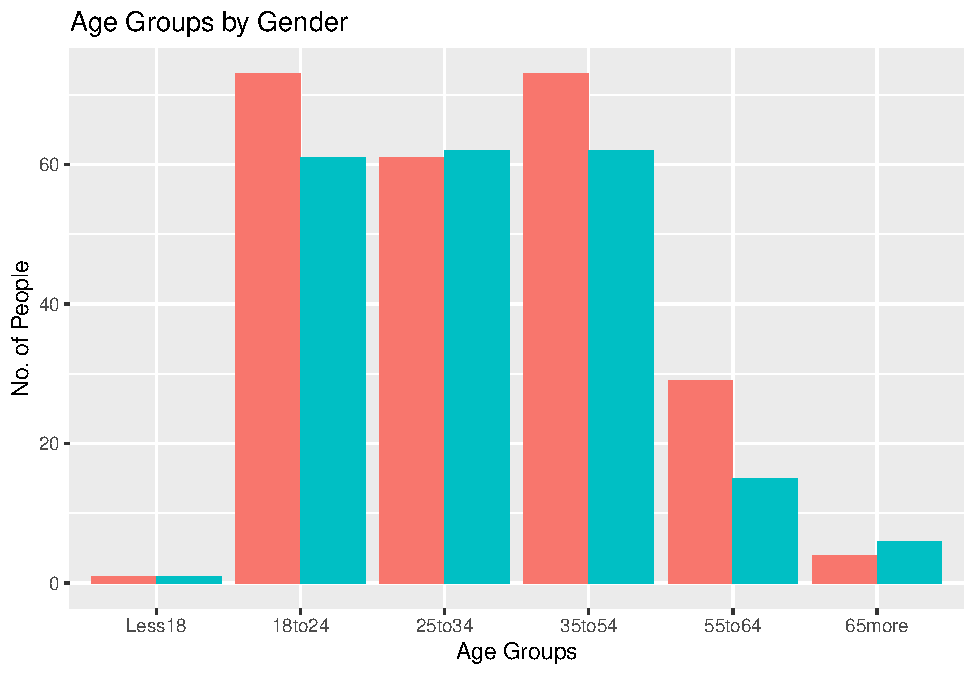
\includegraphics{thesis_files/figure-latex/unnamed-chunk-7-1} 

}

\caption{\label{fig:Education and age by gender}Age Groups by Gender and Education level by Gender}\label{fig:unnamed-chunk-7-1}
\end{figure}
\begin{figure}

{\centering 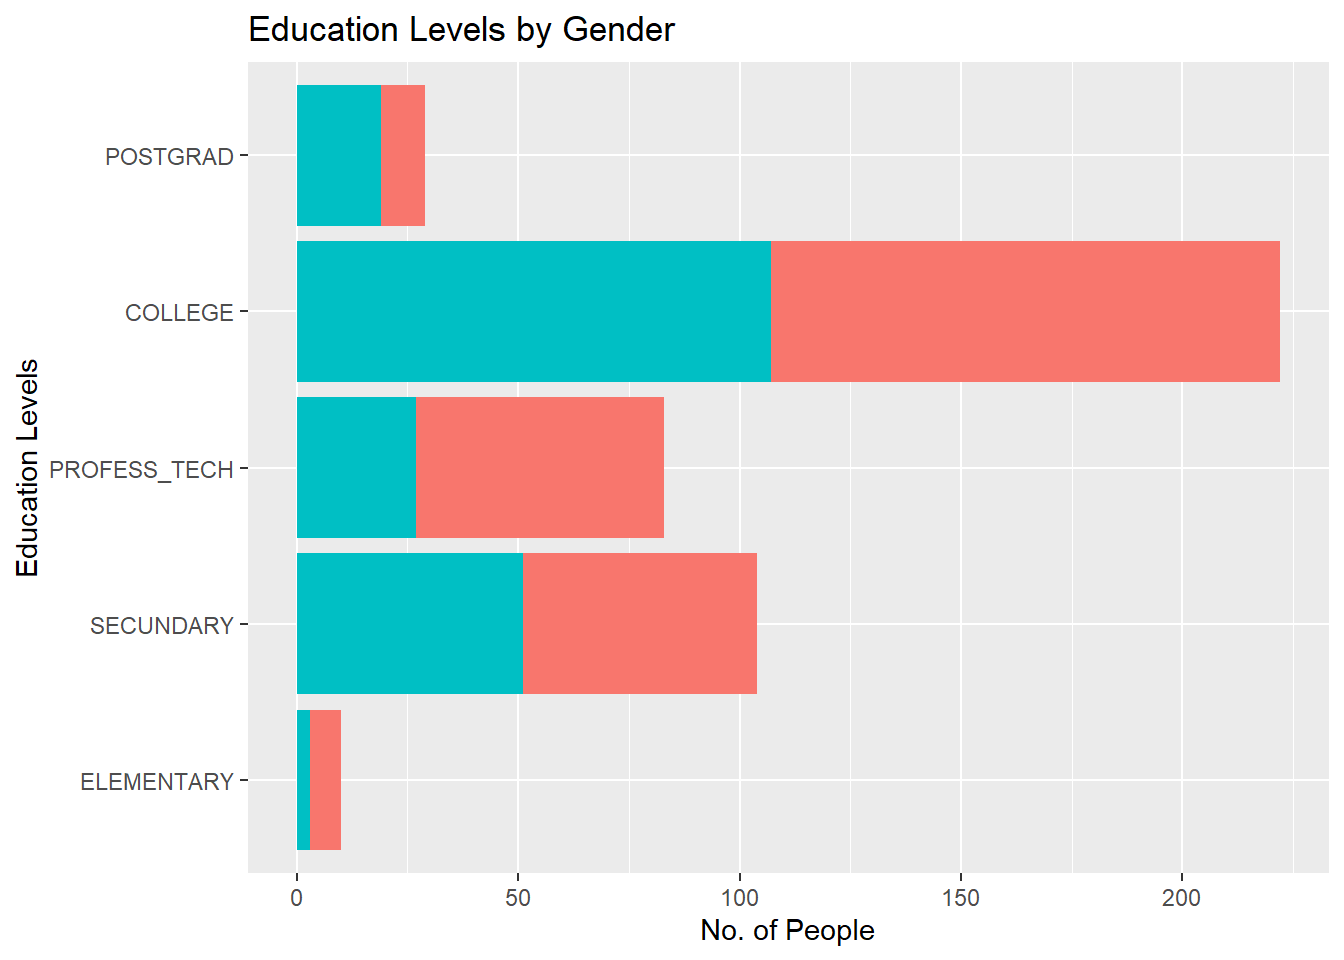
\includegraphics{thesis_files/figure-latex/unnamed-chunk-7-2} 

}

\caption{\label{fig:Education and age by gender}Age Groups by Gender and Education level by Gender}\label{fig:unnamed-chunk-7-2}
\end{figure}
\begin{figure}

{\centering 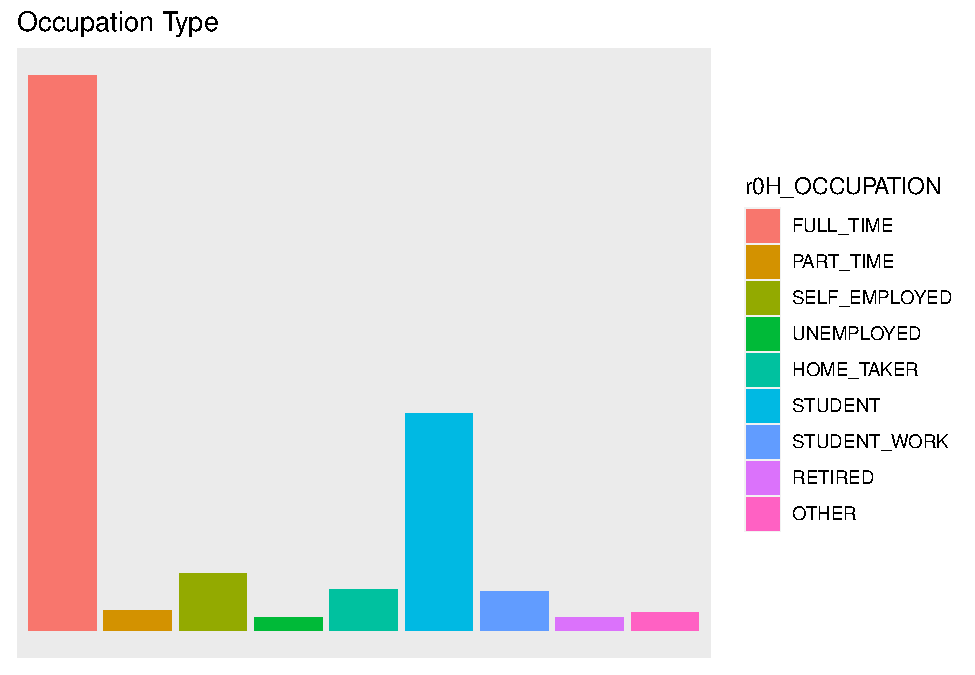
\includegraphics{thesis_files/figure-latex/unnamed-chunk-8-1} 

}

\caption{\label{fig:Occupation type graph}Occupation Types}\label{fig:unnamed-chunk-8}
\end{figure}
The theme of the next table, \texttt{Santiago\_TW}, deals with commuting and work variables (see Table \ref{tab:Travel-work-Descriptive}) and consists of seven ordinal categorical variables (factors). Variable \texttt{r8A\_ACCESSJOB} refers to the impact that respondents feel the transportation network has affected their chances of having better jobs. The most common responses were \texttt{SOME\ IMPACT} and \texttt{NO\ IMPACT}, but we see that approximately 14.2\% of respondents feel that the network has had a major impact.

This variable tracks to some extent with the responses to job opportunities in the commune of residence (\texttt{r8B\_JOBOPP}), suggesting a possible correlation between local opportunities and the impact of the transportation network on job outcomes. When asked about their ideal level of accessibility in the commune of the residence (\texttt{r8C\_ACC\_COM}), a majority respondents opt for excellent and very good.

In terms of the level of satisfaction with their current job, we see that almost 60\% of respondents are at least highly satisfied. We also see that long commutes are frequent in this sample, with about one third or respondents spending 1 h or more travelling and about one quarter of respondents spending between 40 minutes and one hour in their daily commute. This distribution is noteworthy because time spent commuting has been recognized as a factor that can affect physical and mental health and well-being in particular in association with motorized transportation (Brutus, Javadian, \& Panaccio, 2017).

The most common time of the day for commuting is between 7 am and 9 am, but there are also 171 missing responses in this column, so not much can be read from it. Finally, we note that many people spend 35,000-75,000 monthly on their transportation expenditure.
\begin{table}

\caption{\label{tab:unnamed-chunk-10}\label{tab:Travel-work-Descriptive}Variables regarding the commuting behavior of respondents}
\centering
\resizebox{\linewidth}{!}{
\fontsize{12}{14}\selectfont
\begin{tabular}[t]{llrrlrl}
\toprule
skim\_type & skim\_variable & n\_missing & complete\_rate & factor.ordered & factor.n\_unique & factor.top\_counts\\
\midrule
factor & r8A\_ACCESSJOB & 15 & 0.9667406 & TRUE & 5 & SOME IMPACT: 124, NO IMPACT : 123, MINOR IMPACT: 66, MAJOR IMPACT: 64\\
factor & r8B\_JOBOPP & 11 & 0.9756098 & TRUE & 5 & GOOD: 169, POOR: 86, FAIR: 85, VERY GOOD: 64\\
factor & r8C\_ACC\_COM & 15 & 0.9667406 & TRUE & 5 & EXCELLENT: 184, VERY GOOD: 109, GOOD: 93, FAIR: 27\\
factor & r8D\_EMPLSATISF & 37 & 0.9179601 & TRUE & 5 & HIGH SATISF: 135, VERY HIGH SATISF: 130, MEDIUM SATISF: 116, LOW SATISF: 20\\
factor & r8E\_TIMECOMMUT & 10 & 0.9778271 & TRUE & 4 & 1h and more : 133, 40-60 min: 113, 20-40 min: 103, 0-20 min: 92\\
\addlinespace
factor & r8F\_SCHEDULE & 171 & 0.6208426 & TRUE & 6 & 7:00 - 9:00: 168, Others: 47, 9:00 - 13:00: 39, 18:00 - 21:00: 14\\
factor & r8G\_SPENDING & 7 & 0.9844789 & TRUE & 4 & 35,000-75,000: 199, LESS THAN 35,000: 166, 75,000-125,000: 46, MORE THAN 125,000: 33\\
\bottomrule
\end{tabular}}
\end{table}
Table \texttt{Santiago\_SI} includes five variables that capture various aspects of social interaction while commuting (see Table \ref{tab:Social-Interaction-Descriptives}). Social interaction is a topic of interest for mode-related choices given earlier evidence that for some commuters privacy is an important consideration and/or a way to manage social stressors (Gardner \& Abraham, 2007; Lowe \& Mosby, 2016; Páez \& Whalen, 2010).

When asked to rate the level of interaction with other people during their usual trips, respondents In terms of the level of interaction people have with others during their usual trips, most of them presume a good level and they moderately feel it is important when they consider the presence of other people during their usual travels (\texttt{r4A\_INTERACC}) a plurality of responses are ``POOR'' or ``FAIR'' (187) and only 73, that is 16.2\% of respondents, rate their level of interaction as ``GOOD'' or ``EXCELLENT'' report poor or fair (there are 13 missing responses).

With respect to the presence of other people during their travels, the responses tend to be somewhat more ambivalent, and the difference between those for whom this is less or more important is smaller (157 responses are ``NOT'' or only ``SLIGHTLY IMPORTANT'' whereas 132 responses are ``IMPORTANT'' or ``VERY IMPORTANT'').

The next two variables in this table deal with feelings and the experience of discrimination: ``have you felt discriminated against while travelling?'' (\texttt{r4C\_DISCRIM}) and if so, ``while using which mode of transportation'' (\texttt{r4D\_MODE}).

We can see in Table \ref{tab:Social-Interaction-Descriptives}, that slightly fewer than one quarter of respondents (24.2\%) report having felt discriminated while commuting (only 4 responses are missing), and of those close to half (44\%) had that experience in public transportation (however, note that about 58\% of those who felt discriminated against did not state the mode).
\begin{table}

\caption{\label{tab:unnamed-chunk-11}\label{tab:Social-Interaction-Descriptives}Variables regarding social interactions of respondents}
\centering
\resizebox{\linewidth}{!}{
\fontsize{8}{10}\selectfont
\begin{tabular}[t]{llrrlrl}
\toprule
skim\_type & skim\_variable & n\_missing & complete\_rate & factor.ordered & factor.n\_unique & factor.top\_counts\\
\midrule
factor & r4A\_INTERACC & 13 & 0.9711752 & TRUE & 5 & GOOD: 178, FAIR: 102, POOR: 85, VERY GOOD: 53\\
factor & r4B\_PERSON & 12 & 0.9733925 & TRUE & 5 & MODERATELY IMPORTANT: 150, NOT IMPORTANT: 88, IMPORTANT: 83, SLIGHTLY IMPORTANT: 69\\
factor & r4C\_DISCRIM & 4 & 0.9911308 & FALSE & 2 & NO: 338, YES: 109\\
factor & r4D\_MODE & 377 & 0.1640798 & FALSE & 7 & BUS: 33, METRO: 15, CAR: 8, TAXI: 7\\
\bottomrule
\end{tabular}}
\end{table}
The information, telecommunications and mode shifting of respondents (see Table \ref{tab:ITC-Shifting-Descriptives}) reveals numerous factorial variables using Likert scale to identify the exact level of respondents' viewpoints. We can see a considerable number of missing values in quality of changing mode of travel because of people's decision on mostly saying yes to shift between transport modes on their usual trips and for those who change the quality of these inerchanges was good.

Many people assign a good level when they are asked to assess the waiting times, time of shifts and total travel time in their regular trips. Most people have access to technology tools such as smartphones and internet, with which they can view information on transportation services and they assign a good level of technological information available to see transportation alternatives (eg smartphone applications, internet, signs) and most of them assume it is very important to have access to technological information for their usual trips.

This section will gives insights on designing a strong transportation network to facilitate people's different activities such as work, school, grocery shopping and so forth. Also experts can make users informed about traffic circumstances, road information and cost of transportation by using various modes.

Following this, car-use deduction has been turned into the political agenda around the world due to the increasing negative effects of motorized modes of travel on environment and public health. Therefore, improvements in public transportation sector are needed to achieve this goal regarding previous studies that has shown participants are more likely to use bus with increased frequencies, shorter travel time, and high access to bus stops(Ettema et al., 2011).
\begin{table}

\caption{\label{tab:unnamed-chunk-13}\label{tab:ITC-Shifting-Descriptives}Variables regarding information and telecommunications and mode shifting of respondents}
\centering
\resizebox{\linewidth}{!}{
\fontsize{8}{10}\selectfont
\begin{tabular}[t]{llrrlrl}
\toprule
skim\_type & skim\_variable & n\_missing & complete\_rate & factor.ordered & factor.n\_unique & factor.top\_counts\\
\midrule
factor & r6A\_SHIFT & 11 & 0.9756098 & FALSE & 2 & YES: 247, NO: 193\\
factor & r6B\_QUALITY\_SHIFT & 198 & 0.5609756 & TRUE & 5 & GOOD: 107, FAIR: 61, VERY GOOD: 38, POOR: 34\\
factor & r6CA\_WAITING & 41 & 0.9090909 & TRUE & 5 & GOOD: 124, POOR: 101, FAIR: 94, VERY GOOD: 61\\
factor & r6CB\_TIME\_SHIFT & 102 & 0.7738359 & TRUE & 5 & GOOD: 126, FAIR: 77, POOR: 62, VERY GOOD: 59\\
factor & r6CC\_TOTALTIME & 28 & 0.9379157 & TRUE & 5 & GOOD: 138, POOR: 113, FAIR: 75, VERY GOOD: 54\\
\addlinespace
factor & r6D\_DIFFICULTY & 76 & 0.8314856 & FALSE & 7 & ALL THE PREVIOUS ONES: 107, TOO LONG SHIFTS: 89, UNCOMFORTABLE SHIFTING: 87, BAD INFRASTRUCTURE FOR WAITING TIMES: 33\\
factor & r6E\_TOOL & 8 & 0.9822616 & FALSE & 2 & YES: 372, NO: 71\\
factor & r6F\_INFO & 15 & 0.9667406 & TRUE & 5 & GOOD: 153, VERY GOOD: 118, FAIR: 63, EXCELLENT: 63\\
factor & r6G\_IMP\_INFO & 10 & 0.9778271 & TRUE & 5 & VERY IMPORTANT: 198, IMPORTANT: 122, MODERATELY IMPORTANT: 68, SLIGHTLY IMPORTANT: 33\\
\bottomrule
\end{tabular}}
\end{table}
The theme of table \texttt{Santiago\_BE} is perceptions of the built environment. The way environments are perceived, and not just their objective attributes, has been shown to correlate with travel behavior (e.g., Jamal, Mohiuddin, \& Paez, 2020). Surveying perceptions is therefore a good remedy to the lack of canonical data sets in regions of the world where built environment attributes are not systematically collected.

There are in total 22 variables in this table, and their descriptive statistics appear in (see Table \ref{tab:Built-Environment-Descriptives}). The variables are organized in pairs: one asks about the perception of an attribute and the second the importance of that attribute to the respondent.

In this way, \texttt{r7AA\_AUTOSPACE} is about the perception of space for autos, and \texttt{r7BA\_AUTOSPACE} is about the importance that respondents assign to this attribute. Aspects of the built environment covered by this table, in addition to space for autos, are number of parking spaces, quality of highways, space for pedestrians, quality of sidewalks, cleanliness of bus stops and seating areas, protection from inclement weather at bus stops, amount and quality of cycleways, and bike sharing schemes.

The descriptive statistics suggest that most respondents have positive evaluations of space for cars and parking spaces, at the same time that they assign a high level of importance to these attributes. Respondents also show a slight tendency to assess positively the space for pedestrians and quality of sidewalks located near of their home, and these features are also regarded as very important or important by a majority of respondents. In contrast, although respondents feel strongly about the importance of facilities related to buses and cycling, the perception of these attributes tends to be poor.
\begin{table}

\caption{\label{tab:unnamed-chunk-14}\label{tab:Built-Environment-Descriptives}Variables regarding the built environment at the place of residence of respondents}
\centering
\resizebox{\linewidth}{!}{
\fontsize{8}{10}\selectfont
\begin{tabular}[t]{llrrlrl}
\toprule
skim\_type & skim\_variable & n\_missing & complete\_rate & factor.ordered & factor.n\_unique & factor.top\_counts\\
\midrule
factor & r7AA\_AUTOSPACE & 10 & 0.9778271 & TRUE & 5 & GOOD: 127, VERY GOOD: 117, FAIR: 72, EXCELLENT: 67\\
factor & r7AB\_PARKING\_NUMB & 10 & 0.9778271 & TRUE & 5 & GOOD: 119, FAIR: 96, VERY GOOD: 88, POOR: 85\\
factor & r7AC\_QHIWAY & 11 & 0.9756098 & TRUE & 5 & VERY GOOD: 142, GOOD: 141, FAIR: 67, EXCELLENT: 49\\
factor & r7AD\_PEDESTRN & 10 & 0.9778271 & TRUE & 5 & GOOD: 141, VERY GOOD: 102, FAIR: 82, EXCELLENT: 68\\
factor & r7AE\_QSIDEWA & 9 & 0.9800443 & TRUE & 5 & GOOD: 119, FAIR: 110, VERY GOOD: 99, POOR: 67\\
\addlinespace
factor & r7AF\_CLEAN\_STOP & 9 & 0.9800443 & TRUE & 5 & POOR: 129, FAIR: 108, GOOD: 102, VERY GOOD: 67\\
factor & r7AG\_SEAT & 9 & 0.9800443 & TRUE & 5 & POOR: 142, FAIR: 122, GOOD: 94, VERY GOOD: 53\\
factor & r7AH\_CLIMA & 10 & 0.9778271 & TRUE & 5 & POOR: 156, FAIR: 139, GOOD: 88, VERY GOOD: 36\\
factor & r7AI\_CICLEWA\_NUMB & 9 & 0.9800443 & TRUE & 5 & POOR: 189, FAIR: 96, GOOD: 84, VERY GOOD: 37\\
factor & r7AJ\_CICLEWA\_Q & 9 & 0.9800443 & TRUE & 5 & POOR: 171, FAIR: 96, GOOD: 96, VERY GOOD: 44\\
\addlinespace
factor & r7AK\_BICSHARE & 9 & 0.9800443 & TRUE & 5 & POOR: 177, GOOD: 100, FAIR: 69, EXCELLENT: 49\\
factor & r7BA\_IMPAUTOSPACE & 12 & 0.9733925 & TRUE & 5 & VERY IMPORTANT: 140, MODERATELY IMPORTANT: 104, IMPORTANT: 95, SLIGHTLY IMPORTANT: 56\\
factor & r7BB\_IMPPARKING\_NUMB & 12 & 0.9733925 & TRUE & 5 & VERY IMPORTANT: 152, MODERATELY IMPORTANT: 102, IMPORTANT: 91, SLIGHTLY IMPORTANT: 51\\
factor & r7BC\_IMPQHIWAY & 11 & 0.9756098 & TRUE & 5 & VERY IMPORTANT: 214, IMPORTANT: 100, MODERATELY IMPORTANT: 82, NOT IMPORTANT: 23\\
factor & r7BD\_IMPPEDESTRN & 11 & 0.9756098 & TRUE & 5 & VERY IMPORTANT: 278, IMPORTANT: 103, MODERATELY IMPORTANT: 41, NOT IMPORTANT: 10\\
\addlinespace
factor & r7BE\_IMPQSIDEWA & 11 & 0.9756098 & TRUE & 5 & VERY IMPORTANT: 297, IMPORTANT: 86, MODERATELY IMPORTANT: 35, SLIGHTLY IMPORTANT: 12\\
factor & r7BF\_IMPCLEAN\_STOP & 11 & 0.9756098 & TRUE & 5 & VERY IMPORTANT: 286, IMPORTANT: 92, MODERATELY IMPORTANT: 39, SLIGHTLY IMPORTANT: 13\\
factor & r7BG\_IMPSEAT & 11 & 0.9756098 & TRUE & 5 & VERY IMPORTANT: 258, IMPORTANT: 92, MODERATELY IMPORTANT: 56, SLIGHTLY IMPORTANT: 19\\
factor & r7BH\_IMPCLIMA & 11 & 0.9756098 & TRUE & 5 & VERY IMPORTANT: 296, IMPORTANT: 83, MODERATELY IMPORTANT: 34, SLIGHTLY IMPORTANT: 14\\
factor & r7BI\_IMPCICLEWA\_NUMB & 11 & 0.9756098 & TRUE & 5 & VERY IMPORTANT: 296, IMPORTANT: 76, MODERATELY IMPORTANT: 42, SLIGHTLY IMPORTANT: 19\\
\addlinespace
factor & r7BJ\_IMPCICLEWA\_Q & 11 & 0.9756098 & TRUE & 5 & VERY IMPORTANT: 308, IMPORTANT: 67, MODERATELY IMPORTANT: 44, NOT IMPORTANT: 11\\
factor & r7BK\_IMPBICSHARE & 12 & 0.9733925 & TRUE & 5 & VERY IMPORTANT: 259, IMPORTANT: 78, MODERATELY IMPORTANT: 66, SLIGHTLY IMPORTANT: 22\\
\bottomrule
\end{tabular}}
\end{table}
Table \texttt{Santiago\_H} contains responses to twelve questions related to health.
Health information could be useful in investigating affects of transportation policy decisions on public health. Also being aware of specific factors making modes stressful will help transportation and public health experts make commuting a safer, more enjoyable and less stressful activity. Consequently ,planners and transportation experts could mitigate the potentially serious health outcomes of a stressful commute (Legrain et al., 2015). Having such a detailed data set and understanding the relationship between health and mode choice in commuting would help them to adopt reform policies and management strategies in accordance with healthy modes of travel as active and public transportation (Mattisson et al., 2018).

Similar to the set of questions about the built environment, these questions have two parts: first, the respondents were asked to assess their experience of some aspect of their commute, and then the importance they assign to this aspect of their commute.

For example, variable \texttt{r1A\_STRESS} refers to the level of stress that respondents experience in their usual trips; its companion variable is \texttt{r1GA\_IMPSTRESS}, which refers to how important stress is to their experience. As seen in (see Table \ref{tab:Health-Information-Descriptives}), a majority of respondents rate the stress in their commutes as medium or lower.

This aspect of the experience is rated as very important or important by a majority of respondents. Other variables in this table contain information about the physical effort involved in their usual trips (\texttt{r1B\_EFFORT} and \texttt{r1GB\_IMPEFFORT}); proximity to other travelers in their usual trips (\texttt{r1C\_PROX} and \texttt{r1GC\_IMPPROX}); the environmental pollution they are exposed to in their usual trips (\texttt{r1D\_CONTAM} and \texttt{r1GD\_IMPCONTAM}); how safe they feel in their usual trips (\texttt{r1E\_SAFETY} and \texttt{r1GE\_IMPSAFETY}); and finally how comfortable their trips are (\texttt{r1F\_COMFORT} and \texttt{r1GF\_IMPCOMFORT}).
\begin{table}

\caption{\label{tab:unnamed-chunk-15}\label{tab:Health-Information-Descriptives}Variables regarding health information of respondents}
\centering
\resizebox{\linewidth}{!}{
\fontsize{8}{10}\selectfont
\begin{tabular}[t]{llrrlrl}
\toprule
skim\_type & skim\_variable & n\_missing & complete\_rate & factor.ordered & factor.n\_unique & factor.top\_counts\\
\midrule
factor & r1A\_STRESS & 2 & 0.9955654 & TRUE & 5 & MOD: 145, LOW: 107, HIGH: 92, VERY HIGH: 54\\
factor & r1B\_EFFORT & 2 & 0.9955654 & TRUE & 5 & NEUTRAL: 152, POSITIVE: 117, VPOSITVE: 72, NEGATIVE: 67\\
factor & r1C\_PROX & 8 & 0.9822616 & TRUE & 5 & POOR: 130, GOOD: 103, FAIR: 95, EXCELLENT: 60\\
factor & r1D\_CONTAM & 4 & 0.9911308 & TRUE & 5 & VDISSATISFIEDISFIEDSATISFIEDISFIED: 149, DISSATISFIEDISFIED: 138, UNSURE: 107, SATISFIED: 33\\
factor & r1E\_SAFETY & 1 & 0.9977827 & TRUE & 5 & UNSURE: 121, DISSATISFIEDISFIED: 110, VDISSATISFIEDISFIEDSATISFIEDISFIED: 97, SATISFIED: 84\\
\addlinespace
factor & r1F\_COMFORT & 1 & 0.9977827 & TRUE & 5 & VDISSATISFIEDISFIEDSATISFIEDISFIED: 111, DISSATISFIEDISFIED: 109, UNSURE: 103, SATISFIED: 73\\
factor & r1GA\_IMPSTRESS & 6 & 0.9866962 & TRUE & 5 & VERY IMPORTANT: 243, IMPORTANT: 108, MODERATELY IMPORTANT: 57, SLIGHTLY IMPORTANT: 26\\
factor & r1GB\_IMPEFFORT & 5 & 0.9889135 & TRUE & 5 & VERY IMPORTANT: 156, MODERATELY IMPORTANT: 121, IMPORTANT: 102, SLIGHTLY IMPORTANT: 46\\
factor & r1GC\_IMPPROX & 7 & 0.9844789 & TRUE & 5 & VERY IMPORTANT: 169, IMPORTANT: 130, MODERATELY IMPORTANT: 97, SLIGHTLY IMPORTANT: 29\\
factor & r1GD\_IMPCONTAM & 4 & 0.9911308 & TRUE & 5 & VERY IMPORTANT: 258, IMPORTANT: 86, MODERATELY IMPORTANT: 64, SLIGHTLY IMPORTANT: 23\\
\addlinespace
factor & r1GE\_IMPSAFETY & 5 & 0.9889135 & TRUE & 5 & VERY IMPORTANT: 311, IMPORTANT: 80, MODERATELY IMPORTANT: 35, SLIGHTLY IMPORTANT: 13\\
factor & r1GF\_IMPCOMFORT & 5 & 0.9889135 & TRUE & 5 & VERY IMPORTANT: 216, IMPORTANT: 111, MODERATELY IMPORTANT: 91, SLIGHTLY IMPORTANT: 15\\
\bottomrule
\end{tabular}}
\end{table}
First part of the data set of feelings and emotions (see Table \ref{tab:Feelings-Emotions-Descriptives}) reveals factorial variables that people consider them pertained to a specific mode of travel. In terms of freedom, health and social interactions most of people mention them related to walking as a transportation mode. Many people consider using bus connected to unsafety, poverty, unpunctuality, congestion and uncomfortale conditions variables.In terms of using car as the mode of travel, most of respondents identified it connected to functionality, safety, luxury and status.

A large group of people declare that bike riding would be related to enjoyment, low-cost and environment care. The only efficiency variable is being connected to using metro as the mode of transportation in respondents' opinions. In the second part of this table people evaluate the level of enjoy when they are traveling to their daily activities and most of them use average level for this variable and revealed the quality of their trips are very low which is not satisfying. Totally in this table we have half of respondents' answer and the other half is missing values in all variables.

feelings and emotions information can be used to mapping and understanding travel behavior and would lead to a more sustainable transportation network. Additionally, this information can make policy makers aware to make targeted choices about where to make physical amelioration as well as on which characteristics to attempt to influence perceptions of alternative modes(Anable \& Gatersleben, 2005). Similarly, by trying to identify a correlation between feelings, emotions and modes of transportation, planners would be able to persuade people to use more active modes of travel or public transport will be resulted in making our transportation system more sustainable.
\begin{table}

\caption{\label{tab:unnamed-chunk-16}\label{tab:Feelings-Emotions-Descriptives}Variables regarding feelings and emotions of respondents}
\centering
\resizebox{\linewidth}{!}{
\fontsize{8}{10}\selectfont
\begin{tabular}[t]{llrrlrl}
\toprule
skim\_type & skim\_variable & n\_missing & complete\_rate & factor.ordered & factor.n\_unique & factor.top\_counts\\
\midrule
factor & r2AA\_FREEDOM & 218 & 0.5166297 & FALSE & 8 & WALK: 96, CAR: 79, BICYCLE: 43, MOTO: 8\\
factor & r2AB\_UNSAFETY & 217 & 0.5188470 & FALSE & 8 & BUS: 94, MOTO: 73, WALK: 22, BICYCLE: 21\\
factor & r2AC\_FUNCTIONALITY & 196 & 0.5654102 & FALSE & 8 & CAR: 90, MOTOO: 86, BICYCLE: 26, MOTO: 18\\
factor & r2AD\_ENJOYMENT & 212 & 0.5299335 & FALSE & 8 & BICYCLE: 118, CAR: 42, WALK: 42, MOTO: 15\\
factor & r2AE\_LOWCOST & 232 & 0.4855876 & FALSE & 8 & BICYCLE: 91, WALK: 84, BUS: 15, MOTO: 11\\
\addlinespace
factor & r2AF\_POVERTY & 166 & 0.6319290 & FALSE & 8 & BUS: 139, WALK: 102, BICYCLE: 13, COLECTIVO: 10\\
factor & r2AG\_SAFETY & 142 & 0.6851441 & FALSE & 8 & CAR: 199, METRO: 62, TAXI: 16, WALK: 15\\
factor & r2AH\_WASTE\_OF\_TIME & 165 & 0.6341463 & FALSE & 8 & BUS: 222, METRO: 13, CAR: 12, WALK: 12\\
factor & r2AI\_UNPUNCTUALITY & 139 & 0.6917960 & FALSE & 7 & BUS: 263, METRO: 13, WALK: 11, CAR: 10\\
factor & r2AJ\_CONGEST & 233 & 0.4833703 & FALSE & 8 & BUS: 135, CAR: 52, METRO: 16, TAX: 5\\
\addlinespace
factor & r2AK\_EFFICIENCY & 196 & 0.5654102 & FALSE & 8 & METRO: 94, CAR: 63, BICYCLE: 37, MOTO: 17\\
factor & r2AL\_LUXURY & 162 & 0.6407982 & FALSE & 7 & CAR: 200, TAXI: 66, BICYCLE: 8, MOTO: 6\\
factor & r2AM\_ENVIRONMENT & 251 & 0.4434590 & FALSE & 8 & BICYCLE: 121, WAL: 52, METRO: 16, CAR: 4\\
factor & r2AN\_HEALTH & 259 & 0.4257206 & FALSE & 7 & WAL: 94, BICYCLE: 76, CAR: 12, TAXI: 3\\
factor & r2AO\_INTSOCI & 224 & 0.5033259 & FALSE & 8 & WAL: 84, BUS: 41, METRO: 30, BICYCLE: 27\\
\addlinespace
factor & r2AP\_UNCOMFT & 221 & 0.5099778 & FALSE & 8 & BUS: 134, METRO: 51, COLECTIVO: 15, MOTO: 14\\
factor & r2AQ\_HAPPINESS & 216 & 0.5210643 & FALSE & 8 & BICYCLE: 77, WALK: 77, CAR: 65, MOTO: 6\\
factor & r2AR\_STATUS & 173 & 0.6164080 & FALSE & 7 & CAR: 219, TAXI: 28, BICYCLE: 10, WALK: 10\\
factor & r2B\_DAILY\_ENJOY & 4 & 0.9911308 & TRUE & 5 & MEDIUM: 146, HIGH: 114, VERY High: 75, LOW: 72\\
factor & r2C\_IMP\_QUALITY & 6 & 0.9866962 & TRUE & 5 & VERY LOW: 276, LOW: 99, MEDIUM: 46, HIGH: 14\\
\addlinespace
factor & r2D\_AFFECT & 38 & 0.9157428 & FALSE & 8 & ALL OF THEM: 136, TRAVEL TIME: 89, CROWDNESS OF PASSENGERS: 87, COMFORT ABSENCE: 38\\
factor & r2E\_FACILIT & 34 & 0.9246120 & FALSE & 8 & ALL OF THEM: 164, REDUCTION OF TIME TRAVEL: 82, LESS CROWDNESS OF PASSENGERS: 66, BETTER QULALITY ON STREETS: 36\\
\bottomrule
\end{tabular}}
\end{table}
Table of decision-making and planning of respondents (see Table \ref{tab:Reason-Planning-Decision-Descriptives}) includes different factorial variables using Likert scale and has two parts of an assessment of a variable and its importance from respondents' viewpoints. Most of people assign level of good when they assess their access to employment opportunities through public transport and presume a good level about their access to public transport which allows them to access the employment they need.

While people sometimes visit family and friends, do recreational, cultural and sport activities, and they assign a moderate importance to them, most of them often go for grocery/food shopping and social activities and consider it moderately important. In terms of options most of people assume it is very important to have several options in using different modes of transport and they assign very high when they consider quality of life depends on the access they currently have to public transport. Also most people highly think their quality of life would increase if they have better access to public transport.About the affordability and unaffordability of a mode of travel, a large group of people assign car and taxi to these variables, respectively.

For different aspects of the public transport system most of people mention that it has very importance for them to improve access to offices and commercial areas, disponibility of different transport modes, comfort for the use of public transport and the incorporation of other modes to the fare system. Almost all the variables are fairly complete except being economic and uneconomic variables which nearly half of respondents reacted to them.

The most important role of the transportation network and public modes of travel is to provide people with access to different destination in order to travel for business, reuniting with other people, doing grocery shopping and so on. This data set gives us a wide range of variables helpful for identifying people's travel pattern and what level of importance do people assign.So it would be useful for transport-related experts to have an insight about people movement to provide network system with a an appropriate level of performance to increase the efficiency and promote urban transportation system.
\begin{table}

\caption{\label{tab:unnamed-chunk-17}\label{tab:Reason-Planning-Decision-Descriptives}Variables regarding decision-making and planning of respondents}
\centering
\resizebox{\linewidth}{!}{
\fontsize{8}{10}\selectfont
\begin{tabular}[t]{llrrlrl}
\toprule
skim\_type & skim\_variable & n\_missing & complete\_rate & factor.ordered & factor.n\_unique & factor.top\_counts\\
\midrule
factor & r3A\_ACCESS & 11 & 0.9756098 & TRUE & 5 & GOOD: 186, FAIR: 91, VERY GOOD: 63, POOR: 57\\
factor & r3B\_ACC\_EM & 18 & 0.9600887 & TRUE & 5 & GOOD: 134, POOR: 108, VERY GOOD: 83, FAIR: 60\\
factor & r3CA\_FAM & 11 & 0.9756098 & TRUE & 5 & SOMWTIMEs: 117, OFTEN: 105, ALWAYS: 100, NEVER: 60\\
factor & r3CB\_REC & 15 & 0.9667406 & TRUE & 5 & SOMWTIMEs: 139, OFTEN: 103, ALWAYS: 72, RARELY: 65\\
factor & r3CC\_CUL & 14 & 0.9689579 & TRUE & 5 & SOMWTIMEs: 129, RARELY: 123, NEVER: 94, OFTEN: 65\\
\addlinespace
factor & r3CD\_SPO & 15 & 0.9667406 & TRUE & 5 & SOMWTIMEs: 112, NEVER: 106, RARELY: 93, OFTEN: 75\\
factor & r3CE\_GROC & 14 & 0.9689579 & TRUE & 5 & OFTEN: 135, SOMWTIMEs: 112, ALWAYS: 83, RAR: 65\\
factor & r3CF\_SOC & 13 & 0.9711752 & TRUE & 5 & OFTEN: 146, SOMWTIMEs: 107, ALWAYS: 84, RAR: 55\\
factor & r3DA\_FAM & 45 & 0.9002217 & TRUE & 5 & MODERATELY IMPORTANT: 102, IMPORTANT: 85, NOT IMPORTANT: 79, VERY IMPORTANT: 74\\
factor & r3DB\_REC & 47 & 0.8957871 & TRUE & 5 & MODERATELY IMPORTANT: 121, IMPORTANT: 91, SLIGHTLY IMPORTANT: 67, NOT IMPORTANT: 64\\
\addlinespace
factor & r3DC\_CUL & 52 & 0.8847007 & TRUE & 5 & MODERATELY IMPORTANT: 117, IMPORTANT: 87, SLIGHTLY IMPORTANT: 70, NOT IMPORTANT: 67\\
factor & r3DD\_SPO & 50 & 0.8891353 & TRUE & 5 & MODERATELY IMPORTANT: 111, NOT IMPORTANT: 85, IMPORTANT: 77, SLIGHTLY IMPORTANT: 65\\
factor & r3DE\_GROC & 46 & 0.8980044 & TRUE & 5 & MODERATELY IMPORTANT: 101, IMPORTANT: 91, NOT IMPORTANT: 75, VERY IMPORTANT: 70\\
factor & r3DF\_SOC & 47 & 0.8957871 & TRUE & 5 & MODERATELY IMPORTANTORTANT: 124, IMPORTANT: 89, NOT IMPORTANT: 64, SLIGHTLY IMPORTANT: 64\\
factor & r3E\_OPTIONS & 1 & 0.9977827 & TRUE & 5 & NOT IMPORTANT: 326, IMPORTANT: 75, MODERATELY IMPORTANT: 36, SLIGHTLY IMPORTANT: 8\\
\addlinespace
factor & r3F\_ACCESS\_DEPENDENCY & 3 & 0.9933481 & TRUE & 5 & VERY HIGH: 184, HIGH: 128, MEDIUM: 100, BELOW AVERAGE: 21\\
factor & r3G\_QUALITY\_INCRS & 2 & 0.9955654 & TRUE & 5 & VERY HIGH: 267, HIGH: 97, MEDIUM: 54, BELOW AVERAGE: 18\\
factor & r3H\_ECON & 339 & 0.2483370 & FALSE & 8 & CAR: 30, ALL: 30, METRO: 18, BUS: 18\\
factor & r3I\_NOECON & 261 & 0.4212860 & FALSE & 9 & TAXI: 106, CAR: 39, MOTO: 29, COLECTIVO: 4\\
factor & r3JA\_OFIC & 20 & 0.9556541 & TRUE & 5 & NOT IMPORTANT: 195, IMPORTANT: 109, MODERATELY IMPORTANT: 82, SLIGHTLY IMPORTANT: 34\\
\addlinespace
factor & r3JB\_MODES & 17 & 0.9623060 & TRUE & 5 & NOT IMPORTANT: 297, IMPORTANT: 91, MODERATELY IMPORTANT: 38, SLIGHTLY IMPORTANT: 6\\
factor & r3JC\_COMFORT & 14 & 0.9689579 & TRUE & 5 & NOT IMPORTANT: 300, IMPORTANT: 96, MODERATELY IMPORTANT: 34, SLIGHTLY IMPORTANT: 6\\
factor & r3JD\_OTHERS & 20 & 0.9556541 & TRUE & 5 & NOT IMPORTANT: 267, IMPORTANT: 82, MODERATELY IMPORTANT: 51, SLIGHTLY IMPORTANT: 16\\
\bottomrule
\end{tabular}}
\end{table}
It can be seen there are different variables in nature and sustainability table (see Table \ref{tab:Nature-Nustainability-Descriptives}) more through using Likert scale to organize respondents' answer to variables.We can see lots of missing values for changing the mode because most of people do not tend to change their main mode of travel when it comes to a climatic event like heavy rain or flood and for whom wants to change, using car has the most priority.

Most of people have poor level of access to the currently available sustainable modes of transport (eg hybrid buses, electric cars, public bicycles) and they assign high level of importance to that. Again we have so many missing value in payment variable because almost half of people would be willing to spend more on transportation to gain access to more sustainable modes and they indicate 5-15\% of their payments they tend to spend in this regard.In terms of level of importance of improving different aspects in public transport routes most respondents assume high level of importance to presence of trees, access to parks, access to sustainable transport modes and broaden supply of sustainable transport modes.

Nature and sustainability information will helps planner to provide people with a safe, convenient and environment-friendly transportation system. This will also boost the quality of life, people's mobility and goods and enhance economic growth through efficient transportation services. Moreover policy makers would put in place environmental laws and excessive charges for personal car use and ownership (Alyavina, Nikitas, \& Njoya, 2020).
\begin{table}

\caption{\label{tab:unnamed-chunk-18}\label{tab:Nature-Nustainability-Descriptives}Variables regarding perspectives about nature and sustainability of respondents}
\centering
\resizebox{\linewidth}{!}{
\fontsize{8}{10}\selectfont
\begin{tabular}[t]{llrrlrl}
\toprule
skim\_type & skim\_variable & n\_missing & complete\_rate & factor.ordered & factor.n\_unique & factor.top\_counts\\
\midrule
factor & r5A\_CHANGE & 6 & 0.9866962 & FALSE & 2 & NO: 256, YES: 189\\
factor & r5B\_CHANGE\_MODE & 284 & 0.3702882 & FALSE & 8 & CAR: 79, METRO: 34, TAXI: 27, COLECTIVO: 13\\
factor & r5C\_SUST & 7 & 0.9844789 & TRUE & 5 & POOR: 189, FAIR: 97, GOOD: 86, VERY GOOD: 42\\
factor & r5D\_IMP\_SUST & 6 & 0.9866962 & TRUE & 5 & VERY IMPORTANT: 195, IMPORTANT: 115, MODERATELY IMPORTANT: 86, NOT IMPORTANT: 26\\
factor & r5E\_PAYMENT & 6 & 0.9866962 & FALSE & 2 & YES: 228, NO: 217\\
\addlinespace
factor & r5F\_PAYMENTS & 236 & 0.4767184 & TRUE & 2 & 5-15\%: 144, 15-30\%-: 71, 30\% or more\%: 0\\
factor & r5GA\_TREE & 16 & 0.9645233 & TRUE & 5 & VERY IMPORTANT: 236, IMPORTANT: 91, MODERATELY IMPORTANT: 74, NOT IMPORTANT: 19\\
factor & r5GB\_PARK & 12 & 0.9733925 & TRUE & 5 & VERY IMPORTANTORTANT: 254, IMPORTANT: 106, MODERATELY IMPORTANT: 58, SLIGHTLY IMPORTANT: 11\\
factor & r5GC\_MODE & 11 & 0.9756098 & TRUE & 5 & VERY IMPORTANT: 236, IMPORTANT: 105, MODERATELY IMPORTANT: 63, SLIGHTLY IMPORTANT: 25\\
factor & r5GD\_MODE & 11 & 0.9756098 & TRUE & 5 & VERY IMPORTANT: 258, IMPORTANT: 102, MODERATELY IMPORTANT: 48, SLIGHTLY IMPORTANT: 22\\
\bottomrule
\end{tabular}}
\end{table}
\hypertarget{experimental-design-materials-and-methods}{%
\section{Experimental Design, Materials and Methods}\label{experimental-design-materials-and-methods}}

The study is based on a paper-based survey conducted face-to-face in Santiago in 2016. The survey collected information on a wide range of travel-related issues (socio-demographics, health-related, perceptions and travel behavior, travel choices and planning, social interaction factors, built environment, among others).

The data collection considered a quota-sampling method based on the information from Pre-Census of 2012, and in total, 451 persons validly completed the survey. This paper considers the first part of the survey, with information about the basic socio-economic data, travel choices, activities and commuting information, and the question related to the levels of stress experienced in while traveling.

\hypertarget{is-your-commute-like-a-bad-boss-learned-helplessness-and-normalization-of-stress-in-the-commute-experience-in-santiago}{%
\chapter{Is your commute like a bad boss? Learned helplessness and normalization of stress in the commute experience in Santiago}\label{is-your-commute-like-a-bad-boss-learned-helplessness-and-normalization-of-stress-in-the-commute-experience-in-santiago}}

\hypertarget{introduction-3}{%
\section{Introduction}\label{introduction-3}}

Travel essentially could have an advantage which can be different from reaching a destination or for achieving a goal. It has been suggested that travel does not necessarily belong exclusively to the second layer of activities; instead, it can form an activity of its own, as observed in undirected travels driven by a sense of speed, motion, and control. Moreover, people may undertake excess travel even combined with mandatory trips and do not try to make it reasonable in accordance with the target of travel. Other psychological aspects like the joy and relaxation may have an important role from their viewpoint (Mokhtarian \& Salomon, 2001).

According to people's target of travel, they assign importance on two types of psychological motives namely as instrumental (environment, cost, health and fitness, convenience, predictability, flexibility) and affective (Relaxation, no stress, excitement, control, freedom).

For instance, if they are traveling for a leisure time, they expect more freedom, convenience and low level of stress. For work trips, while active modes users were satisfied with these motives almost equally, users of motorised modes are satisfied with instrumental factors with higher rate than affective factors. For these kinds of users, convenience and flexibility may outweigh affective factors such as stress as previous study has shown (Anable \& Gatersleben, 2005).

This can be a kind of normalization because people try to adjust what they are struggling with and focus on other related dimensions to the problem. But there is a question: Should they do this in only life-threading conditions, or it works also in non-life-threading conditions? Previous work has shown that if people use normalization in non-life-threading condition it may impair the level of their quality of life.

(Koslowsky, 1997) found that commuting experience may be accompanied by work-related stressors . Interestingly, People are different in their sensitivity and vulnerability to stressful events (Shamoa-Nir \& Koslowsky, 2010). At high risk of experiencing stress, people are in danger of feeling psychological problems and sleep disturbance.

Individuals who perceived themselves as physically weak had higher rates of mental health problems. This would be an apparent sign of the importance that people would assign to conditions in which they feel psychological problems leading to lose their self-esteem, face with self doubt and feel stress. The unremitting stress could trigger psychological issues of anxiety, fear, panic attacks, post traumatic stress symptoms, psychological distress, stigma, avoidance of contact, depressive tendencies, sleep disturbances, helplessness and interpersonal social isolation depending on their profession.

In some cases, the correlation between psychological resilience level and the perceived stress level is turned out to be reverse in a way that they may feel more resilient to the psychological effects like stress and they perceive less stress level. It can be seen in some positions Fear of labeling, stigmatization and discrimination potentially impede workers intent to seek counselling and psycho therapeutic interventions. Despite the common mental health problems and psycho social issues among workers in such settings, most of them do not often seek or receive a systematic mental health care.

According to a theory based on Lazarus and his colleagues, stress is perceived as a relationship between an individual and the environment relevant to its well being in which they have positive or negative evaluation. Having this feeling, cognitive appraisal has two parts: first a person can decide whether the encounter is irrelevant, benign-positive or stressful. In second part the person will measure coping resources and alternatives, try to address his/her question about what they should do in this situation. These parts work interdependently in a way that if coping strategies are considered as enough resources, the threat of the event will diminish and vice versa.

Emotions are of importance as people interpret their perceptions toward what is going on in an environment. As a diagnostic tool, emotions are vital because their intensity and quality determine how people organize the feeling of importance to them and this has a direct relation with their evaluation of a happening.

In general, coping strategies has two majors namely as cognitive and behavioral besides a broad range of functions to handle a problematic situation between a person and an environment. First major is centered around the control of agitating emotions which is more practical when the encounter is unchangeable from a person's perception (emotion-based coping).

Some kinds of emotion-based coping strategies are identified as diminishing threat, seeking emotional or social support, wishful thinking and self-blame. The second one seeks to improve the annoying situation by doing an act (problem-based coping). In contrast, problem-based coping strategies are more popular when the encounter is changeable. In the following paragraphs eight scales of these strategies will be identified by their own characteristics.

Wishful thinking is a way that focuses on how a person is dealing with the problem by thinking about changing the situation or tackle with that like maintaining a normal life, thinking about solutions, maintaining situational control and information seeking. Distancing as the second one refers to trying to forget the whole matter and waiting for what will happen next. Emphasizing the positive would be the third one focusing on considering the bright side of things like using a positive altitude while addressing the issue.

Items four to six contain self-blame (criticizing myself), tension-reduction (trying to make a better feeling by doing favorite behaviors and self-isolation (avoidance of contact with others as the negative copying style and related to high levels of stress. All the others are associated with lower levels). Seventh item is a mix of both problem and emotion-based coping entitled ``Seeking social support'' covers sympathetic feelings and talking to someone else in order to making the situation easier to understand.

This is the one used typically by people more than choosing one form or the other one (Folkman \& Lazarus, 1985). Apart from classification, another kind of emotion-based strategies implies adaptive coping strategies including religion and social support (Babore et al., 2020).

The Last item as a salient statement of problem-based coping strategies would be ``adhere to a plan of actions'' (Folkman \& Lazarus, 1985). Depending on the strategies which people take into account for coping with mobility stress, vulnerability can be indicated. Mobility stress could be a situation in which people are unable to use comfortable means of mobility. Vulnerability means a living situation which is detrimental to psychological condition of people. Regarding this people may adopt strategies such as: travel by non-motorised means, readiness to high fare, cancellation of trips, travel in company of relatives, reduced number of trips, purchase of private automobile (Odufuwa, 2008).

Another coping strategy would be time allowing the individual to control stressors related to time components. Similarly, increasing control or predictability may be influential in this regard. If the commuter can be informed of special situations that exist on the way to work, such as traffic accidents or a closed road, both perception of control and predictability could be enhanced. Interestingly, with the aid of radio station in the morning (in many communities today special radio frequences in the morning and evening report on traffic patterns and even make recommendations on alternative routes) the expected negative effects of commuting can be mitigated. For example, flexitime, telecommuting, and subsidised carpooling are techniques for making the commute easier (Koslowsky, 1997).

The objective of this research is to investigate whether normalization/learned helplessness could be coping strategies, and if so for whom. Data for the research are drawn from a survey conducted in Santiago, Chile, based on a quota-sampling method based on the information from Pre-Census of 2012, and in total, 451 persons validly completed the survey.

The rest of the research is structured as follows.

\hypertarget{background-1}{%
\section{Background}\label{background-1}}

\hypertarget{stress-and-transportation}{%
\subsection{Stress and transportation}\label{stress-and-transportation}}

Generally, stress include a wide variety of factors and there is no single identifier broadly accepted. One of these would be stress caused by commuting. People with any target of travel may face stress while commuting between origins and destinations. Although a broad range of source of stress are identified as commuting stress, they can be primarily classified as two categories of objective stressors and subjective moderators.

As (Koslowsky, 1997) has identified, the first group indicates objectives as impedance like commuting time, distance or speed as a combination of time and distance, and commuting condition such as traffic congestion. Previous studies reveal that length of travel and congestion are strongly related to the increase of stress. People feel less stress when they experience a movement with less possible amount of time and distance.

The concept of commute impedance was specified as a behavioral control on movement or reaching a target. In other words, it contains anything that impose frustration on the goal to be reached at a certain time at a particular place such as distance, slow speed or traffic congestion. Speed would not have direct effect as an impedance, but some other extraneous factors may split from that.

To make a clarification on that we can assume two drivers first driving at 35 mile/hour and second driving at 50 mile/hour. The former one may be driving on local roads, at maximum possible speed and without experiencing any barrier while the former one may be driving on a highway, face congestion (on superhighways like German autobahn) and find negative stimuli on the road. In current study identifying these, help us understand how stressors affect commuters' feeling and mode selection mostly for daily routines.

Based on (Koslowsky, 1997)'s findings, second cluster contains subjective variables like perception of control over the commute (commuting mode), predictability of commuting conditions and personal characteristics namely as gender or family specifications.

While there is no evidence indicating effect of subjective factors, some studies have considered active modes like driving a car or riding a bike which provide more control, are more associated with less stress that passive modes like public transport. On the contrary, another study hypothesize that car users are more at the exposure of stress than bus or train users. Given these, there might be a possibility of other factors like noise or congestion to have effect on perceived stress by different modes of transportation.

As a kind of moderator, predictability of commuting has a significant role in perceived stress on commuting. Commuters capable of predicting the length of travel may face less commuting stress than their counter parts who are uncertain about this. Also, the relation of variability of commute and higher level of commuting stress is evident.

Also, according to (Gottholmseder et al., 2009) there are other factors can be considered to show the effect of stress on commuting such as assessment of commuting time, alcohol consumption, leisure-time activities, and job attributes.

\hypertarget{coping-with-stress-normalization-and-learned-helplessness}{%
\subsection{Coping with stress: Normalization and learned helplessness}\label{coping-with-stress-normalization-and-learned-helplessness}}

Studies have indicated the source of ``Normalization'' as (Benyamini, Gozlan, \& Weissman, 2017) has found the concept of normalization was mostly developed in nursing research on families with chronically ill children. Normalization consists of reducing the feeling of being different and achieving as normal a life as possible, acknowledging the existence of the impairment (which distinguishes it from denial), using a normalcy lens to define the situation, constructing a story of life as normal and going on to enact it, and carrying on with life activities as if the illness can be ignored. As can be expected, this reaction can be seen among some people while they are suffering from their commute for various reasons, they are going to ignore the negative impact of their experience mentally.

In the context of psychological resilience and perceived stress (Boran, Boran, Korukcu, \& Özkaya, 2022) found that people at high risk of experiencing stress like health workers are in danger of feeling psychological problems and sleep disturbance. By using some scales for instance resilience scale and perceived stress scale including Likert scale, through a survey it has been figured out that to what extent people can tolerate stressful conditions and what is their exact perception of this feeling. It has been stated that individuals who perceived themselves as physically weak had higher rates of mental health problems. This would be an apparent sign of the importance that people would assign to conditions in which they feel psychological problems leading to lose their self-esteem, face with self doubt and feel stress.

While exploring consequences of stress and the way of dealing with that (Rana, Mukhtar, \& Mukhtar, 2020) found that people regarding their profession might be at high risk of anxiety, stress, and depression. The severity is causing further mental health problems which not only effect workers' ability to make decisions, but could also have long term detrimental effect on their overall well-being.

The risk of a sudden change in their roles like being downgraded can lead to psychological problems, such as disappointment, helplessness, adaptation problems, and fear of change. Similar studies like (Webster, Brough, \& Daly, 2016) have shown that people due to helplessness may use some coping strategies such as leaving the stressful situation and asking social support. When individuals feel they are in an uncontrolled situation they are more likely to revert to avoidance-focused coping strategy. Those victims who could not deal with these toxic conditions nor leave may feel learned helplessness and chronic health issues in long term harm. Normalize stress in some situations due to individuals' specific conditions may prevent them to deal with the main stressors.

Similarly (Rana et al., 2020) found that people who are experiencing high stress environment - emotional and behavioral responses would be naturally adaptive while facing the extreme (unpredictable and uncertain) stress, and therefore counselling and psychotherapy based on the stress-adaptation model could be used as an early and prompt intervention . (Maier \& Seligman, 1976) also found that this feeling of helplessness might have origins in uncontrollable factors and people assume their behavior and outcomes are independent and this learning produces the motivational, cognitive and emotional effect of uncontrollability. Learned helplessness will be shown as a defective performance where reduced incentive motivation is undermined.

Similar studies in the context of normalization and coping strategies like (Benyamini et al., 2017) have found that when individuals are in a situation in which they suffer from a (physical) problem, depending on to what extent they have internalized the norms and principles, they might be distressed by unexpected and uncontrollable barriers to its fulfillment. In such conditions, normalization seems to play a significant role by trying to achieve higher levels of quality of life and better adjustment.

But in fact, normalization is weakly related to quality of life. Normalization in long-term impairs quality of life mainly due to its social consequences. On the one hand, normalization in other non-life-threatening chronic or long-term conditions that are known to impair quality of life of young adults as they struggle to attain the developmental milestones reached by their own peers. On the other hand, Normalization includes a focus on other goals in life, instead of or in addition to those that are currently blocked. For example, by adjusting another related goal following failed treatment we can mitigate its effect on.

Nevertheless, people can choose to (re)engage in other goals at the same time. Engaging in alternative meaningful goals has been found to be adaptive for people undergoing serious physical problems, with its effects seen mainly in terms of greater well-being. Normalization, in the sense of maintaining life routines and balancing between the physical and other life domains, allows for such goal re-engagement.

\hypertarget{stress-and-coping-strategies-in-transportation}{%
\subsection{Stress and coping strategies in transportation}\label{stress-and-coping-strategies-in-transportation}}

\hypertarget{stress-and-transportation-1}{%
\subsubsection{Stress and transportation}\label{stress-and-transportation-1}}

Based on commuting stress research as (Koslowsky et al., 2013) has also mentioned, every single commuters may experience various stressors such as standing for whole time on the crowded public transport on hot whether or getting drenched because of a rainstorm while walking back home from public stations to work or home.

As Koslowsky et al. (2013) a typical commuter may experience a wide variety of stressors on the way to and from work such as physiological stressors which also include environmental factors such as noise, crowding. heat and noxious fumes. Other stressors can be time pressures and agressive of reckless behaviors. Thses are just a few examples of the effect of commuting stress on commuters.

The inevitable role of human being in the general chain of traffic issues is taken into consideration as it leads to stress, accident and aberrant behaviors. (Westerman \& Haigney, 2000) have revealed that there would be two predominant classification of Driver Behavior Inventory (DBI) assessing driver stress and Driver Behavior Questionnaire (DBQ) investigating aberrant driver behavior.

Unsatisfying traffic conditions may aggravate the situation and increase frustration on the road leading to high level of stress. Some people would underestimate the risk of confrontation with an accident and tend to overrate their capabilities while driving. While this high level of confidence in vehicle control decreases driver stress level, it would lead people to adopt dangerous attitudes and driving maneuvers requiring specific skills. (beneficial level of stress because it can mediate risk of stress. Stress is generally bad when it is excessive.)

The Driver Behavior Inventory as a measure of driver stress indicates driver stress and performance as a function of evaluating traffic demands, appraising personal competence and selecting coping strategies. According to recent studies of DBI, three main aspects of driver stress vulnerability has been emerged namely as:

-Aggression (i.e., anger, impatience and risk taking which can be addressed through confrontive coping strategies)

-Dislike of driving (i.e., anxiety, self-blame and lack of confidence tackled by self-criticism coping strategies or negative emotions that diverts attention from the driving task)

-Alertness (i.e., awareness of risk and active search for road hazards issued by task-focus (problem solving) coping strategies.

According to a study conducted by (Kontogiannis, 2006), the direct relationship between aggression and self-criticism has been found and reveals aggressive drivers could be aware of their behavior but they cannot take preventive actions. These findings would be beneficial for traffic safety organization looking for reducing aggression on the roads.

According to DBI, there would be two additional categories of driver stress as irritation when overtaken and frustration when overtaking, has been suggested. It seems that these overtaking factors in comparison to the former factors are more predominant on aggression. Following this, two new ``situation-specific'' factors in a five-factor solution were identified. ``Situation-specific'' tension associated with aggression and included two overtaking factors while ``situation-specific'' concentration correlated with alertness but consisted of only two items. Furthermore, confidence factor was recognized based on an extensive questionnaire including a new confidence factor related to control perception.

An interesting relation exits between confidence and violation (aberrant behavior: leading to accident and caused by stress) as people with high record of violations felt more confident about vehicle control. Which is maybe related to the relation among, underrate risk of accident, overrate driving skills, high level of confidence, high possibility of undertaking driving maneuvers.

Finally, new factors of ``fatigue'' and ``thrill seeking'' have been revealing followed by an administration of a questionnaire. Studies within the context of real-world behavior, have revealed high aggression related to faster driving and more risky overtaking. While dislike scale was associated with weaker vehicle control. An interesting study has found men reported higher aggression and comparatively lower overtaking tension. The relations between age and driver stress have indicated older drivers due to declining trend of cognitive capacities experienced high stress and were less alert (Westerman \& Haigney, 2000).

\hypertarget{coping-strategies}{%
\subsubsection{Coping strategies}\label{coping-strategies}}

In stressful traffic situation, individuals should select appropriate actions to cope with stress. As (Kontogiannis, 2006) mentioned before, two general categories of coping strategies have been identified: problem-based and emotion-based.

Problem-focused followers tend to adopt tasks and rational strategies such as:

o Information seeking

o Taking precaution and making plan: Making an action to drive in a safe way such as avoid making risky overtaking and changing route when it is necessary in an appropriate time

o Confrontive coping: Expressing feelings through risk taking like driving close to next car's bumper, beeping, flash light beams on other drivers.

On the contrary, emotion-based drivers appear to regulate emotions and decrease discomfort by different ways such as:

o (Escape avoidance) Avoidance: Trying to suppress negative feelings to overcome the problem

o Wishful thinking

o Reappraisal: Considering driving as a learning experience such as trying oneself to calm down and emphasizing the positive point

o Self-criticism: Criticizing oneself for mistakes such as feeling failure and self-doubt

The adherence of these two broad coping strategies has been recognized diverse and related to individuals' preferences.

Furthermore, studies about chronic stress (DBI scale) and coping behaviors has led to a consistent relationship between them. First dimension implies that drivers revealing anger, frustration and impatience (like aggression scale) were more likely to tackle stress through confrontive coping. Second would be drivers feeling anxiety and fear (like dislike of driving scale) were more interested in opting negative emotional coping styles deviating attention from driving action. Alertness as last dimension and an attribute of active hazard surveillance seems to be addressed by a problem-solving coping strategy. Alertness anticipated speed of discrimination of roadside pedestrians.

To improve the distinction of problem-focused versus emotion-focused coping skills, it is vital to define specific road scenarios and observe how drivers respond to them rather than considering general form of driving which is not enlightening (like slow-driving: someone is driving in front of you making overtaking hard, and discourtesy scenarios: someone is driving behind you near to your rear bumper beeping because . In addition, diversity and socio-cultural backgrounds around the world would affect factor structure of driver stress and its correlation to coping styles.

Previous researches have shown that professional drivers chose a group of both problem-based and emotion-based strategies. This selection may change regarding the level of frustration and anger felt in various road scenarios.

\hypertarget{materials-and-methods}{%
\section{Materials and methods}\label{materials-and-methods}}

The presented data in this article were gathered purposefully through a questionnaire to capture various dimensions of urban living and mobility in a major city in the Global South. Data used to analysis in this research are drawn from a survey conducted in Santiago, Chile, in 2016 using a quota-sampling method based on the information from Pre-Census of 2012, with a total of 451 participants.

The questionnaire covers different topics such as personal characteristics, work-related travel information, and perceptions of the built environment. Other themes include social interactions while using different modes of transportation, mode switching, and the use of information technologies. The questionnaire also addresses several self-reported health outcomes, feelings and emotions related to commuting experiences, attitudes toward transportation system satisfaction, and perceptions of nature and sustainability.

This study focuses on both demographic and health-related information. To assess participants' views on stress during their commute, multiple questions were asked, including variable r1A\_STRESS as one of our dependent variables, which reflects the level of stress experienced during regular trips using a 5-point Likert scale (very low, low, moderate, high, and very high). Its corresponding variable, r1GA\_IMPSTRESS as the other one of our dependent variables, evaluates the importance of stress during commuting and is also assessed using a 5-point Likert scale (not important, slightly important, moderately important, important, and very important).

Furthermore, health information can be useful in understanding the effects of transportation policy decisions on public health. Identifying the specific factors that contribute to stressful modes of transportation can help transportation and public health experts make commuting a safer, more enjoyable, and less stressful experience.

\hypertarget{data-preparation}{%
\subsection{Data preparation}\label{data-preparation}}

Collect the data on the two ordinal variables of interest and check for any missing data or out liners. If necessary, clean the data and re-code it into ordinal categories.

The case study for this research covered the Santiago Metropolitan as Chile's capital and largest city containing various communes as shown (see Figure \ref{fig:study boundaries}). The data-set used in current study obtained from a paper-based survey conducted face-to-face in Santiago in 2016.

The data set contains essential socio-economic and demographic information about the respondents, as well as their built environment and behaviors commuting to work. In addition, the survey (conducted between DATE-DATE, 2016) includes information about the respondents' feelings and emotions in relation to their commuting experience, the social experience of a variety of transportation modes, various self-assessed health questions, patterns of use of information and telecommunication technologies, and questions about sustainability and the environment.

The data collection conducted a quota-sampling method based on the information from Pre-Census of 2012, and in total, 451 participants took part in the survey. This study considers the first two parts of the survey including individual characteristic and health information to figure out the relationship between personal attributes and stress related variables.
\begin{figure}

{\centering 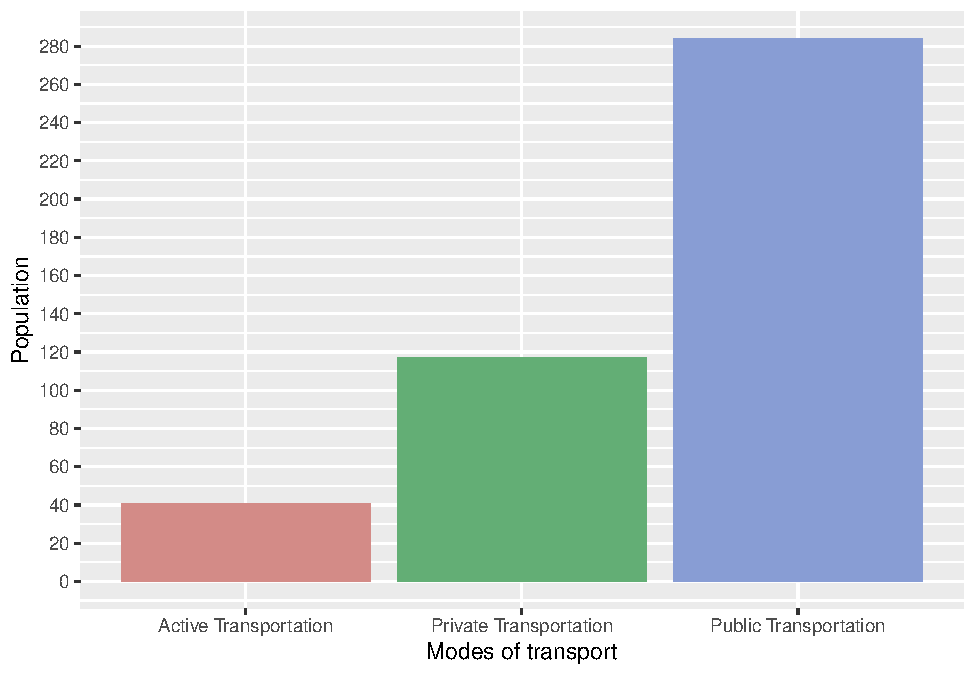
\includegraphics{thesis_files/figure-latex/unnamed-chunk-21-1} 

}

\caption{\label{fig:study boundaries}Santiago the case study}\label{fig:unnamed-chunk-21}
\end{figure}
\hypertarget{variables}{%
\subsection{Variables}\label{variables}}

As mentioned earlier in the study, previous researches have applied various variables for implementing the ordinal regression model. In this study we employ a group of dependent and independent variables extracted from individual characteristics and health information parts of the surveys. As dependent variables we chose stress indicator of level of stress experienced by respondents while commuting and another stress criterion revealing the importance level of the stress experienced when traveling by participants. For independent variables we selected respondents age and income level, occupation, and their primary mode of transportation while regular commuting.

To initialize our bivariate ordinal model, we took advantage of previous studies about the how was the importance of different independent variables withing individual characteristics.

Although gender looked effective on some of driver stress scales like confidence and alertness, it was rather weak to indicate gender difference in terms of coping strategies. Previous studies revealed men feel more confidence and alert that their counter parts. Regarding coping strategies, women seemed to score higher in cognitive strategies despite men who tend to use behavioral strategies. (Kontogiannis, 2006). Although it has been found that women were more likely to feel stress and anxiety that men, some studies has shown that women and men in a rather similar conditions felt the same level of stress (Hill and Ng Boyle, 2007).

Age sounded influential on most of aspects of driver stress vulnerability. Getting older had a positive role in a way that it increased cognitive coping strategies useful in decreasing stress level and declined negative behaviors like aggression (Kontogiannis, 2006), thus they felt less stress.

Another study indicated the relation of age with stress in a completely different way as some situation-specific tensions tend to increase by getting old until some of older ones may decide to not to drive (Hill \& Boyle, 2007). Age also could be negatively related to manifestation of violation and dangerous behaviors as old drivers tend to decrease the speed due to the declining cognitive capabilities (Westerman \& Haigney, 2000).

In contrast of old people, youth were more likely to reveal their driving anger through behavioral coping strategies(Hill \& Boyle, 2007).

Based on findings of previous research on determinants of individual's vulnerability to mobility stress, level of education and family status would be influential on the experienced stress while commuting. Also, high level of income would provide people with the opportunity of purchasing a private vehicle limiting their driving stress and uncomfortable experience with public means (Odufuwa, 2008).

In order to reach the more efficient model we used re-code\_factor() argument which requires the dplyr R package to be loaded, and the function takes the original factor variable as the first argument, followed by the re-coding rules. The re-coding rules in this study are specified using a set of named character vectors to aggregate or disperse the original levels of the factor and the values represent the new levels.

\hypertarget{modelling-approach}{%
\subsection{Modelling approach}\label{modelling-approach}}

One of the most common analysis of ordinal data would be related to modeling the preferences or opinions in various fields. In this regard we can see the application of modelling in correlated ordinal data as multiple outcomes for a number of subjects or objects like participants responding to a questionnaire. Given these multivariate setting, models and particularly multivariate ordinal regression models sound practical to deal with the correlation among ordinal outcomes.

Current study has used similar application of bivariate ordinal regression models (Kenne Pagui \& Canale, 2016) considering the gap between expected satisfaction and experienced service. It refers to two different blocks that participants are asked to say to what extent the service has importance and as the second part they are required to reveal the actual feeling about the given service.

As can be seen in the study conducted by (Hirk, Hornik, \& Gür, 2020) the class of multivariate ordinal regression models implemented in mvord and can be applied to other applications such as having multiple or repeated ordinal observations. This research takes advantage of package mvord for R Studio which provides a flexible framework for analysing correlated ordinal data using the class of multivariate ordinal regression models.

This class of modeling assumes each ordinal response as a categorized version of an underlying continuous latent variable separated based on specific threshold parameters. This flexible framework contributes helps to imposing constraint on thresholds along with regression coefficients using arguments.

In this study we implement bivariate logit link for the class of multivariate ordinal regression models. In terms of identifiability, imposing some restriction on the parameters is needed as the absolute scale and location are not identifiable in ordinal models. Therefore, in order to make the model identifiable, we use one of the options regarding constraining parameter set by the following way:

{[}Fixing the intercept \(\beta_{j0}\) (e.g., to zero), using flexible thresholds \(\theta_j\) and fixing \(\sigma_{ij}\) (e.g., to unity) \(\forall j \in J_i\) and \(forall i \in (1, \cdots, n)\){]}.
(Hirk et al., 2020)

\hypertarget{analysis-and-results}{%
\section{Analysis and results}\label{analysis-and-results}}

In order to fit our bivariate ordinal regression model, we can use mvord R package which has two different data structures of MMO and MMO2. As we are working with wide data format and the covariates stored in different columns of the data set do not change during multiple measurements, using MMO2 data structure is an appropriate way. In this data structure each subject i refers to on row of the data frame and all the covariates are stored in different columns.

At this point we used the following formula to specify the model:

mod\_bivariate \textless- mvord (formula = MMO2(r1A\_STRESS,r1GA\_IMPSTRESS) \textasciitilde{} 0 + r0D\_AGE + r0J\_INCOME + r0P\_MODE1 + r0G\_EDUCATION + r0H\_OCCUPATION ,
link = mvlogit(df = 8L)

where ``mod\_bivariate'' is the name of the model, ``mvord'' is the function for fitting multivariate ordinal models, and ``MMO2'' is the data structure in accordance with wide format of data set. Predicators are demographic variables of the respondents namely as their age, income, education and occupation level as well as their primary mode of commute.

As the second step to make sure of the model identifiability and reveal the latent correlation in the model, we used an argument to constrain the coefficients.

\hypertarget{discussion}{%
\section{Discussion}\label{discussion}}

The results of the model analysis can be seen in Table \ldots{} . The analysis reveals that adult individuals aged between 35 to 54 are the most affected category when it comes to rating the importance stress during commuting. There is a positive correlation indicating that adults within this age range are more likely to assign importance to stress while commuting.

This trend holds until the age of 54, after which seniors aged 55 and above are significantly related to experience stress. The negative coefficient for this age group suggests that their stress level is decreasing compared to their younger counterparts.

This finding may seem incompatible with some previous research claiming that as people get older, they tend to avoid risks and tensions, especially while driving. However, it is important to consider that older individuals may also suffer from cognitive limitations (Westerman \& Haigney, 2000) and have difficulties remembering their lapses, leading to potentially dangerous and stressful situations. This may put them at a higher risk of accidents or unpleasant commuting experiences with more stressful moments. The declining ability to self-monitor and remember specific errors could contribute to this phenomenon (Rabbitt, 1990).

Previous research has indicated that income groups play a significant role in the relationship between travel and satisfaction. It has been suggested that commute satisfaction is associated with commute enjoyment, commute stress, social comparisons, personality, and overall well-being (Ye \& Titheridge, 2019). People with higher incomes are more likely to afford better modes of travel, such as personal drivers, and therefore experience fewer stressful situations.

As it can be seen in the model, the higher income category is strongly associated with a negative and relatively large coefficient, even larger than the middle-income group, indicating less probability of experiencing stress. This could be attributed to their capability or overall well-being, enabling them to choose different modes of transportation to avoid stressful commuting experiences. These individuals may utilize problem-solving or emotion-based coping strategies.

As it has been indicated, the more people drive the less stress they experience as they become accustomed to it and this regularity helps them develop coping strategies and become more adept at the drive (Legrain et al., 2015). Interestingly, the middle-income group, despite having a positive coefficient, does not show a significant association with the experienced stress but it is still positive. However, it is worth noting that this group is highly and positively associated with assigning importance to the experienced stress during commute.

Previous work has also revealed that lower-income groups (can be considered as similar to middle income) rated instrumental factors (e.g., cost, predictability, flexibility) higher than higher income groups (Ye \& Titheridge, 2019). This could explain why lower-income (middle income in our study) individuals are not strongly associated with mentioning the importance of stress. They are more likely to choose public transportation or active modes of transportation due to limited options available to them.

Moreover, it has been indicated that the impact of commuting mode on stress should be considered by transportation and planning agencies in making decisions (Wener \& Evans, 2011). Because commuting specifies level of perceived control over this process which has a reverse relation with stress (Gottholmseder et al., 2009).

According to the current study, both public and private modes of transportation are positively associated with experiencing stress during commutes. Large coefficient indicates a more significant association between experiencing stress and those who choose public and private modes of transportation than active mode users. These findings are compatible with previous work indicating that commuting by car and public transit are considered to be more stressful and boring than active commuting. This has also been revealed that commuting satisfaction is associated with commute stress to a large extent and hence pedestrian, train travelers, and cyclists are significantly more satisfied with their commuting than car drivers, metro and bus users (Ye \& Titheridge, 2019).

Having higher level of education has been found to be associated with a positive and relatively significant coefficient leading to a more probability of assigning importance to the self-reported stress while commuting. As already has been mentioned, commute satisfaction has a strong effect on commute stress, and these are followed by short distance factor(Ye \& Titheridge, 2019). According to a previous study on the effect of tele-work on daily travel in Sweden, people with higher education are more likely to travel longer and this finding is willing to put travelers more at the exposure of experiencing stress (Elldér, 2020).

In terms of occupation, current study has shown that experiencing stress among those who have a profession or students is significantly associated. Negative coefficient for both groups implies that their stress level has a decreasing trend compared to their counterparts. In addition, increasing trend of stress level has been indicated in some professions like construction due to different reasons like having an unsafe workplace or occupational tensions (Loosemore \& Waters, 2004).
\begin{table}

\caption{\label{tab:unnamed-chunk-22}Bivariate ordered model: Estimation Results}
\centering
\resizebox{\linewidth}{!}{
\fontsize{8}{10}\selectfont
\begin{tabular}[t]{llccclccc}
\toprule
  & Equation1 & beta\_equation1 & se\_equation1 & p\_values\_E1 & Equation2 & beta\_equation2 & se\_equation2 & p\_values\_E2\\
\midrule
1 & - & - & - & - & r0D\_AGEAdults 1 & 0.5732 & 0.2105 & <0.0001\\
2 & r0D\_AGESeniors 1 & 0.5732 & 0.2105 & <0.0001 & - & - & - & -\\
3 & r0J\_INCOMEMiddle Income 1 & -0.9002 & 0.2245 & 1e-04 & - & - & - & -\\
4 & - & - & - & - & r0J\_INCOMEMiddle Income 2 & 0.3625 & 0.2049 & <0.0001\\
5 & r0J\_INCOMEHigh Income 1 & -0.6607 & 0.2248 & <0.0001 & - & - & - & -\\
\addlinespace
6 & r0P\_MODE1Private Transportation 1 & 1.4984 & 0.3515 & 0 & - & - & - & -\\
7 & r0P\_MODE1Public Transportation 1 & 1.5199 & 0.3175 & 0 & - & - & - & -\\
8 & - & - & - & - & r0G\_EDUCATIONHigher Education 1 & 1.5149 & 0.7432 & <0.0001\\
9 & r0H\_OCCUPATIONWorking 1 & -0.9825 & 0.3217 & 0 & - & - & - & -\\
10 & r0H\_OCCUPATIONStudent 1 & -0.9821 & 0.3677 & <0.0001 & - & - & - & -\\
\addlinespace
VLOW|LOW & VLOW|LOW & -2.275 & 0.4221 & 0 & NOT IMPORTANT|SLIGHTLY IMPORTANT & -1.9388 & 0.7862 & <0.0001\\
LOW|MODERATE & LOW|MODERATE & -0.7954 & 0.4246 & <0.0001 & SLIGHTLY IMPORTANT|MODERATELY IMPORTANT & -0.6362 & 0.7312 & <0.0001\\
MODERATE|HIGH & MODERATE|HIGH & 0.6368 & 0.4283 & <0.0001 & MODERATELY IMPORTANT|IMPORTANT & 0.4615 & 0.7319 & <0.0001\\
HIGH|VHIGH & HIGH|VHIGH & 1.9855 & 0.4451 & 0 & IMPORTANT|VERY IMPORTANT & 1.6449 & 0.7367 & <0.0001\\
\bottomrule
\end{tabular}}
\end{table}
Regarding analysis during our bivariate ordinal mode, we reclassified different modes of transportation into three general categories of active transportation (walking and cycling), public transportation (taxi, collective, metro and bus) and private transportation (car and motorcycle).

As can be seen (see Figure \ref{fig:Modes of transport}), respondent mostly use public means of transportation with almost 285 out of 451 respondents as their main choice for commuting. Recent studies also have shown that using public transport has formed almost 50\% of motorized trips as a salient example of the popularity of public transportation in Santiago, Chile over the recent years (Pezoa, Basso, Quilodrán, \& Varas, 2023).

Regarding this popularity and to make it more productive, it has been mentioned that public transport in Santiago as a modern and integrated system is called Transantiago referring to a sustainable public transport system for Santiago. By aggregating services such as bus and metro and keeping the fare expenses with a low range, passengers can benefit from an efficient system of transport which was unsuccessful (Muñoz \& Gschwender, 2008) and needs some consideration to work as planners expected.

Following this, second popular mode of transportation can be assigned to private mode with around 25\% of the whole population or 120 persons. Some users also were interested in eco-friendly modes like walking and cycling with slightly more than 40 people and 10 \% of the whole respondents.
\begin{figure}

{\centering 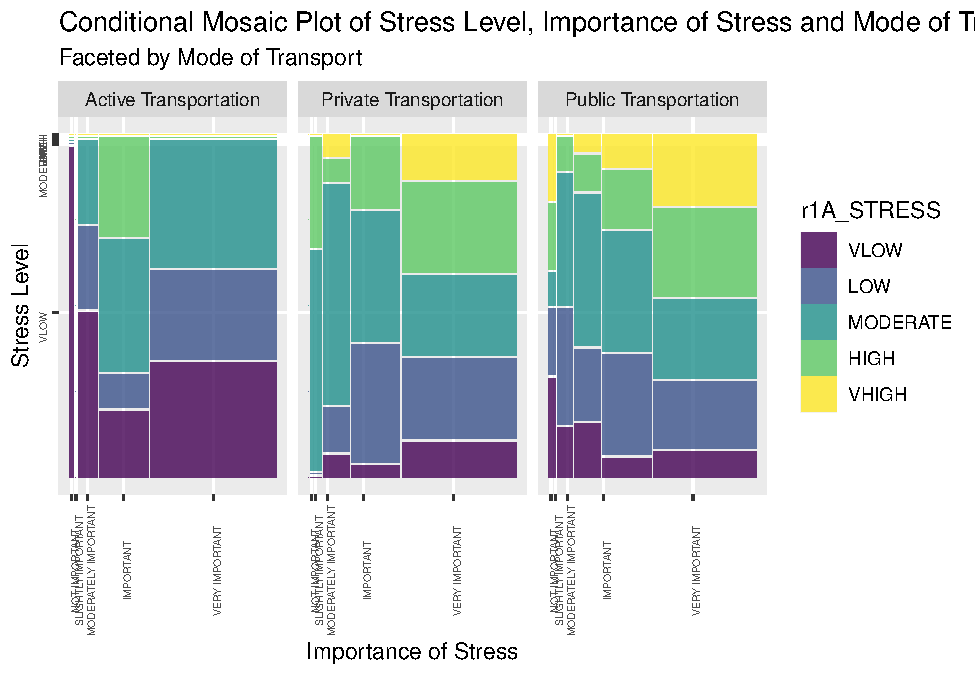
\includegraphics{thesis_files/figure-latex/unnamed-chunk-23-1} 

}

\caption{\label{fig:Modes of transport}Modes of transport}\label{fig:unnamed-chunk-23}
\end{figure}
To have a better understanding of the interaction among the key variables of modes of transportation, age groups, income levels, experienced levels of stress and the importance assigned to the stress, some mosaic plots were adopted.

Mode, age and income are the most crucial variables in our study. As it has been studied in previous work, different modes of commuting can be effective on people's feeling and in general the subjective well-being referring to the importance of focusing on individuals' travel experiences such as stress (Smith, 2017).

Income also is one of the significant variables as it determine people's options for commuting like if they are low income workers they tend to use more public transportation in Santiago, Chile (Gómez-Lobo \& Micco, 2023) which could be important from stress of commute's perspective that can be seen mostly among public transport users in this study. Another influential variable on people's experience of commuting is age which sometimes makes commuting difficult for older people specially when they choose walking according to the folks in La Cisterna district to the city center in Santiago (Tironi \& Palacios, 2016).

So we are analyzing these items in terms of their effect on each other.

According to the results from the cross tabulation of modes of transport by age groups that youth as the most populated age group were interested in using active and more public transport with more than 60\% of each. Following this, adults as the second most populated age group were also interested in using more private and afterwards active mode with almost half of private mode users and 23\% of active mode users, respectively. Apart from this, seniors were mostly interested in private transport with around 15 \% of whole private users and less tend to use active and public with about 10 \% for each of them.

Therefore as can be seen (see Figure \ref{fig:Transportation Mode by Age group}) youth respondents tend to use public and active mode, adults are more interested in private and active, and seniors use almost all modes in a similar way but more interested in private mode.
\begin{figure}
\centering
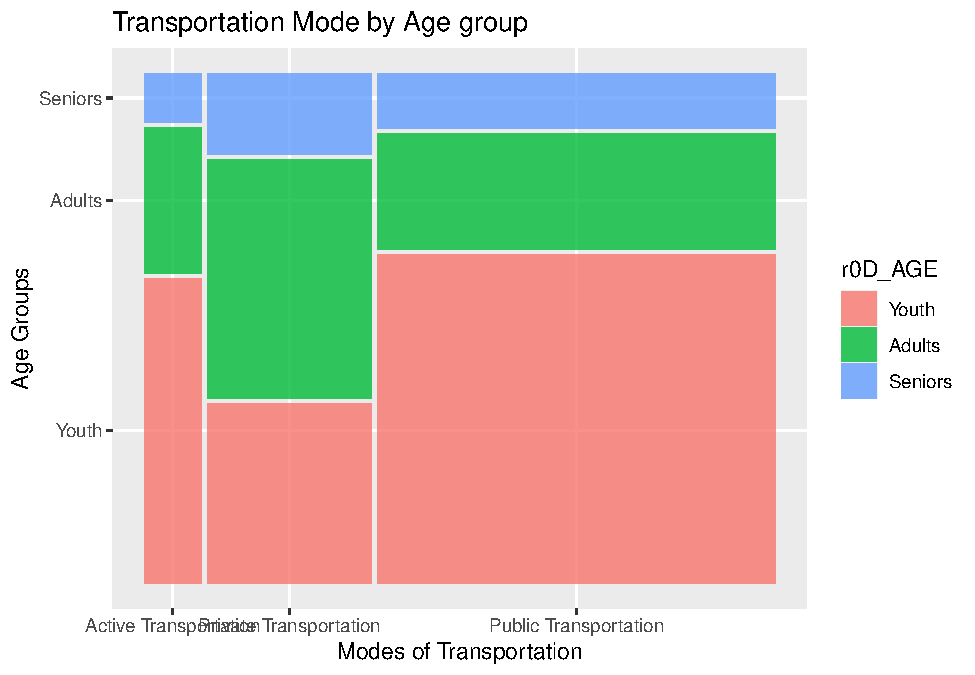
\includegraphics{thesis_files/figure-latex/unnamed-chunk-24-1.pdf}
\caption{\label{fig:unnamed-chunk-24}\label{fig:Transportation Mode by Age group}Transportation Mode by Age group}
\end{figure}
\begin{figure}

{\centering 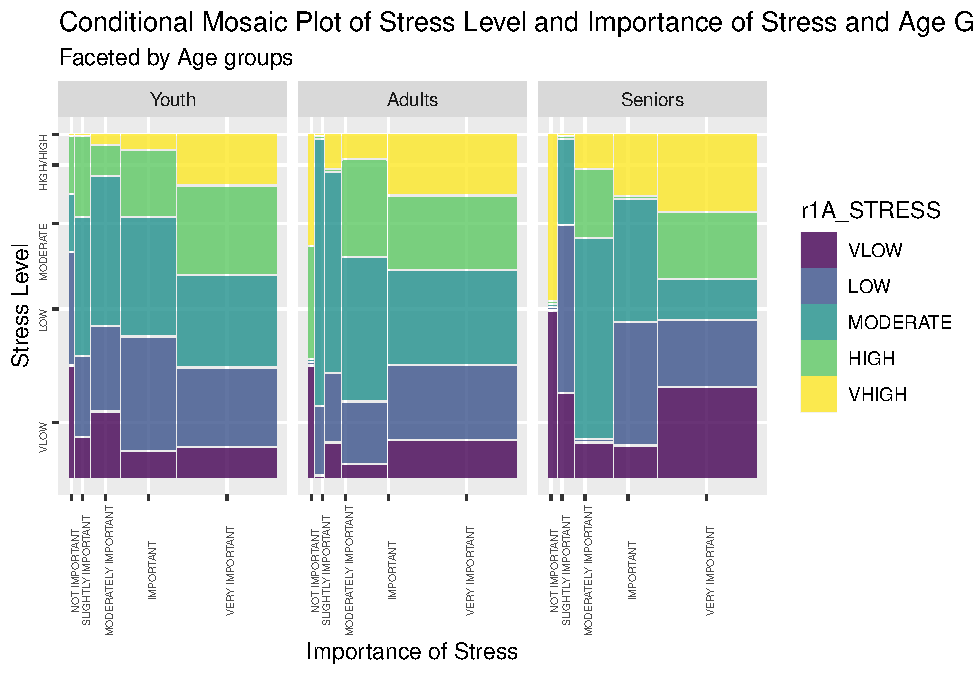
\includegraphics{thesis_files/figure-latex/unnamed-chunk-25-1} 

}

\caption{\label{fig:stress and importance of stress and mode}Conditional Mosaic Plot of Stress Level, Importance of Stress and Mode of Transport}\label{fig:unnamed-chunk-25}
\end{figure}
As (see Figure \ref{fig:stress and importance of stress and mode}) shows that while active users as the least populated mode of transport, felt mostly low levels of commuting stress, they assigned high importance to that and among all, active users had the highest rate of importance.

To be more in details, more than 60\% of those who feel very low and low level of stress, give the highest level of importance to that. Following this an almost opposite trend can be seen for private and public users that when they feel high and very high levels of stress, that sounds so crucial to them to assign highest level of importance to their stress feeling.

According to (see Figure \ref{fig:stress and importance of stress and mode}) almost more than 70 \% of public and private users who felt high and very high level of stress, mentioned that was important to them. Similarly, assigning importance by the rest of these people who felt stress in lower levels slopes to more medium and low levels as the stress level is going to decrease.

It is also an interesting fact that although all users have assigned high levels of importance to the stress, private and public transports users felt relatively higher levels of stress compared to their active mode counter parts. Also, these public and private groups incorporate almost 90\% of the whole respondents.
\begin{figure}
\centering
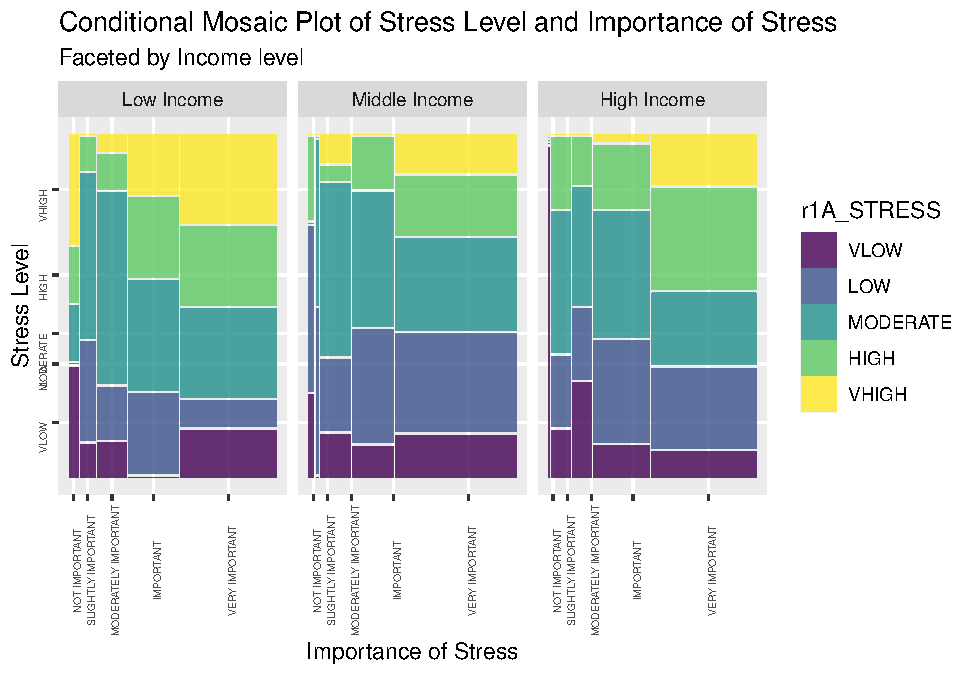
\includegraphics{thesis_files/figure-latex/unnamed-chunk-26-1.pdf}
\caption{\label{fig:unnamed-chunk-26}\label{fig:stress importance of stress and income}Conditional Mosaic Plot of Stress Level, Importance of Stress, and Income Level}
\end{figure}
As (see Figure \ref{fig:stress importance of stress and income}) indicates that people in all of the income groups have assigned high levels of importance to stress when commuting. This trend has been indicated from the table (number) that 80 \% of all groups have assigned important and very important levels on feeling stress when commuting. Moreover, the highest rate of giving high level of importance is associated with middle income group at all feeling stress levels as the most populated group (almost 33\% of the whole respondents).

It is also interesting that among all of the income groups, low income users felt highest level of feeling stress over all of the importance stages. On the contrary, a huge number of people belong to middle level of income (almost 60 \% of the middle group) felt low and moderate levels of experiencing stress and less than 20 \% of them felt high and very high levels of stress of commuting. This can be considered in a similar way for high income level people as well because the largest part of people felt a range of low to high level of stress with almost similar percentages to Middle group.

Generally, while almost all people considered high levels of importance about stress, the larger portion of them including middle and high income felt less challenging ranges of stress in comparison to low income levels.
\begin{figure}
\centering
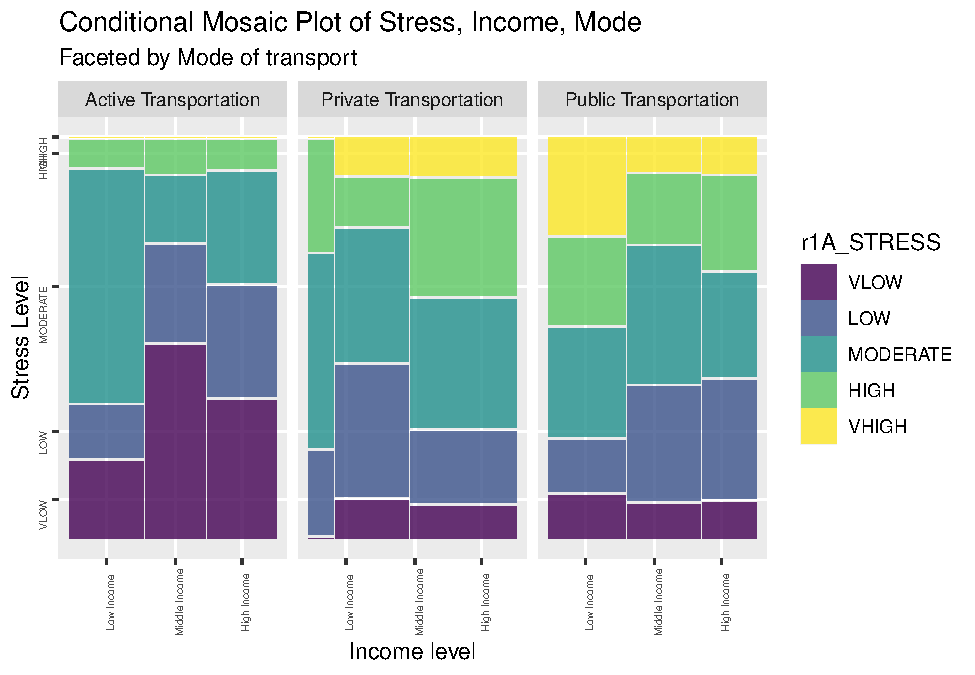
\includegraphics{thesis_files/figure-latex/unnamed-chunk-27-1.pdf}
\caption{\label{fig:unnamed-chunk-27}\label{fig:stress importance of stress and age}Conditional Mosaic Plot of Stress Level and Importance of Stress and Age Groups}
\end{figure}
According to (see Figure \ref{fig:stress importance of stress and age}) youth and adults as the most populated groups incorporate 60\% and 30\% of whole respondents. A common trend among all groups is that around 30\% of them felt moderate stress level and seniors had the largest portion of feeling stress at a very high level compared to other users.

About youth and adults as the larger portion of respondents there is a kind of similar dispersion of feeling stress ranges from low to high level with about more than 70\% of people in both age group For the importance of stress, while almost all groups felt high level of stress, the importance of stress was far more important for adults ,and seniors and youth assigned mostly very high level of importance but slightly less than adults.
\begin{figure}
\centering
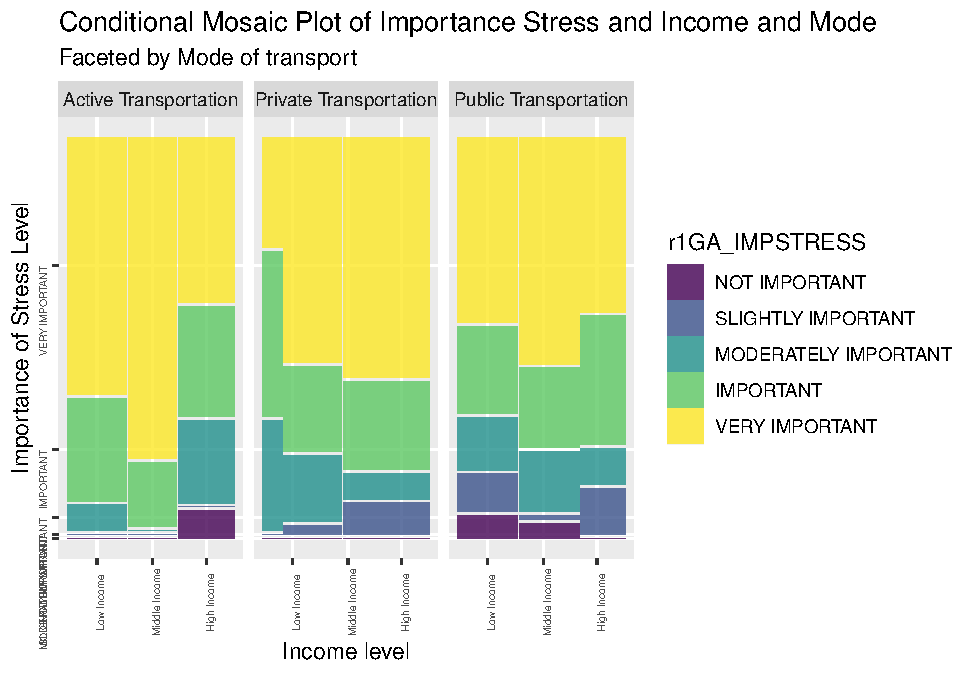
\includegraphics{thesis_files/figure-latex/unnamed-chunk-28-1.pdf}
\caption{\label{fig:unnamed-chunk-28}\label{fig:Income-mode-Age}Conditional Mosaic Plot of Mode, Age and Income}
\end{figure}
The analysis of the data(see Figure \ref{fig:Income-mode-Age}) reveals distinct trends among different age groups in terms of income levels and preferred modes of transportation. The youth category primarily aligns with high income levels and active transportation modes. In contrast, adults show a notable association with middle income, alongside a relatively minor difference in low income, often opting for private modes of transportation.

Among seniors, there's a prevalence of low income status, with a preference for private transportation modes. These findings provide insights into the varying preferences and financial considerations that influence transportation choices across age groups.
\begin{figure}
\centering
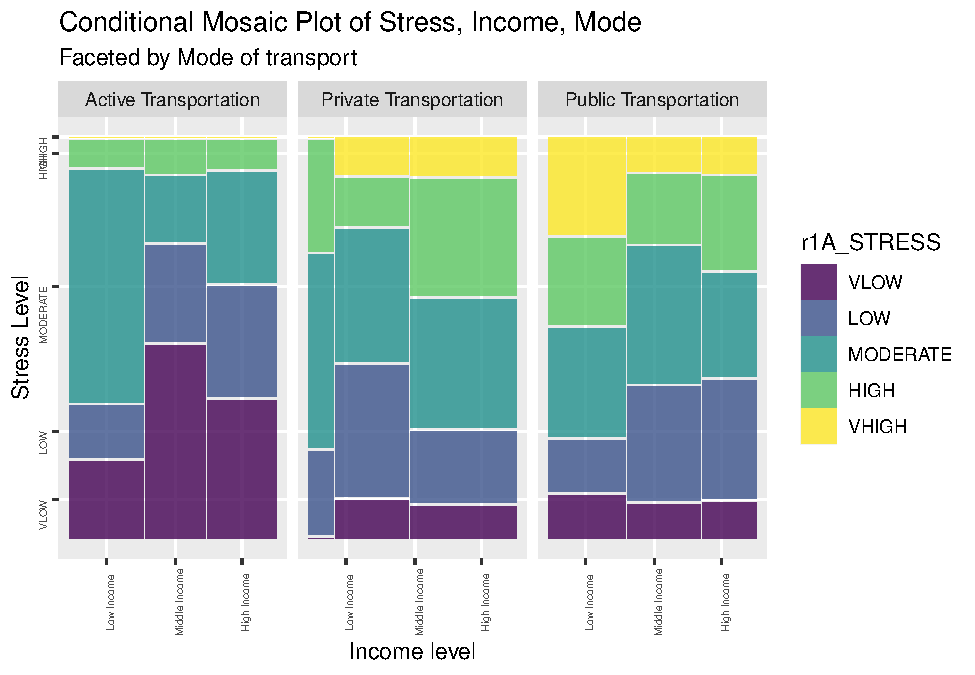
\includegraphics{thesis_files/figure-latex/unnamed-chunk-29-1.pdf}
\caption{\label{fig:unnamed-chunk-29}\label{fig:IMS}Conditional Mosaic Plot of Stress, Income, Mode}
\end{figure}
As it has been revealed (see Figure \ref{fig:IMS}), almost 80\% of lower level income people and 65\% of middle income level as the most populated group use public transport which has been indicated to be highly stressful especially among low income ones. High income respondents where the most interested group in using private mode with 40 \% of them and relatively less commuting stress but they highly rely on public mode with about 50\% among all.
\begin{figure}
\centering
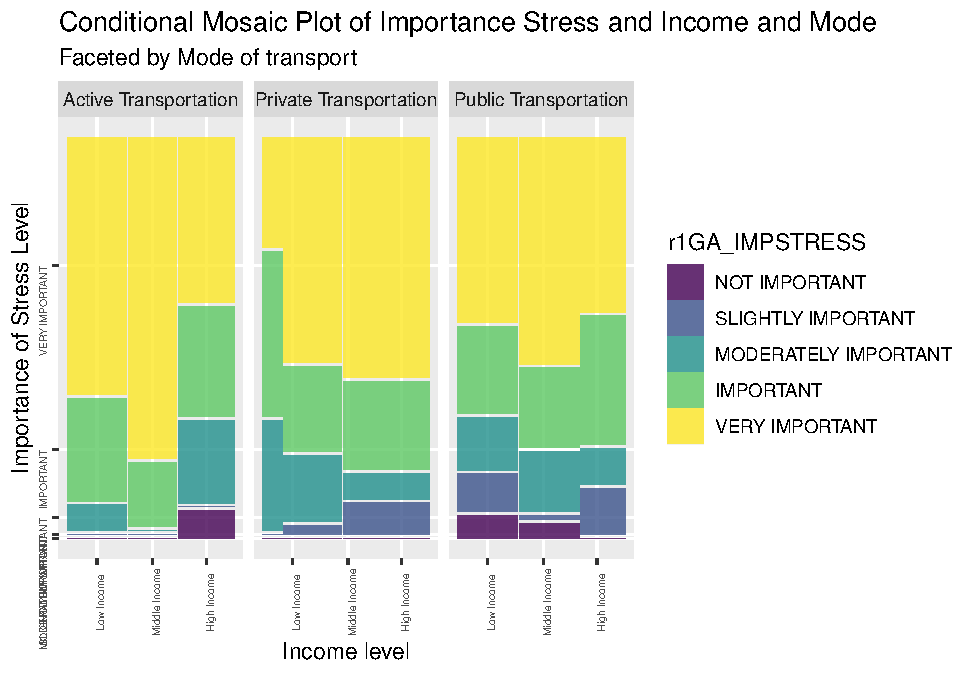
\includegraphics{thesis_files/figure-latex/unnamed-chunk-30-1.pdf}
\caption{\label{fig:unnamed-chunk-30}\label{fig:Income-mode-and-importance-stress}Conditional Mosaic Plot of Importance Stress and Income and Mode}
\end{figure}
The analysis of the provided information reveals (see Figure \ref{fig:Income-mode-and-importance-stress}) distinct patterns within different income groups, stress levels, and transportation modes. Among low-income individuals, the preferred mode of transportation is predominantly public (40.8\%), aligning with a significant prevalence of the ``Moderate'' stress level (37.01\%) and the ``Not important'' stress importance category (37.67\%).

In the middle-income group, ``Active'' transportation is most common (39.2\%), while a majority experiences ``Low'' stress levels (43.2\%). Notably, the ``Very important'' stress category (40.88\%) is prominent. Conversely, high-income individuals tend to favor private transportation modes, coinciding with the highest occurrence of the ``Very high'' stress level (46.3\%). The ``Slightly important'' stress category (75.48\%) also stands out. This comprehensive analysis provides insights into the complex interplay between income, transportation choices, and stress levels and importance of stress.
\begin{figure}
\centering
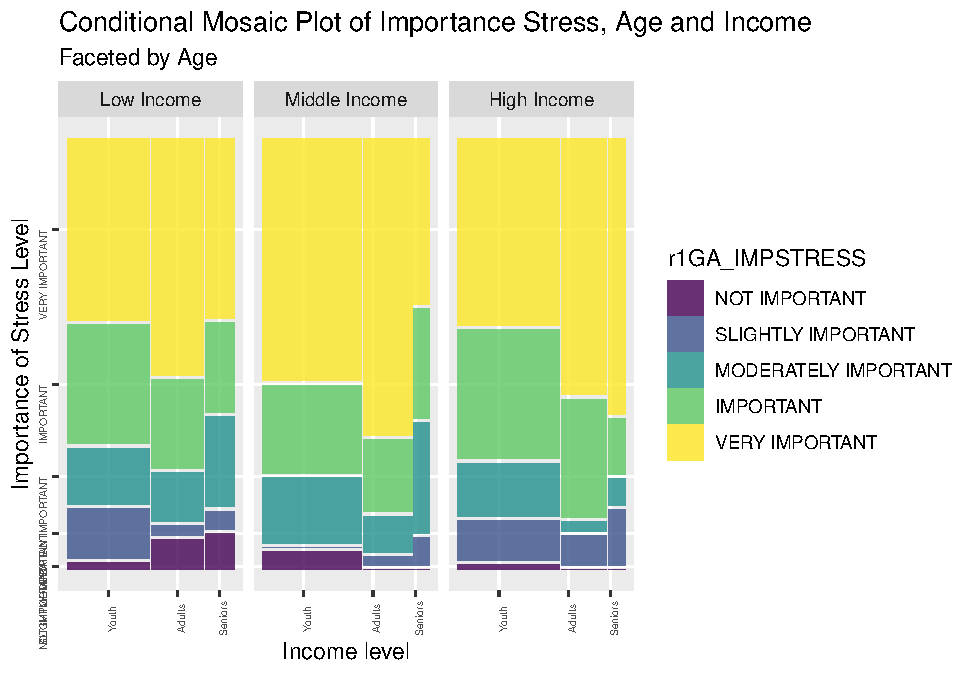
\includegraphics{thesis_files/figure-latex/unnamed-chunk-31-1.pdf}
\caption{\label{fig:unnamed-chunk-31}\label{fig:Income Age and importance of stress}Conditional Mosaic Plot of Importance Stress, Age and Income}
\end{figure}
The analysis of the data (see Figure \ref{fig:Income Age and importance of stress}) categorizes the importance level of stress in association with income and age groups. Middle-income youth, as well as low-income adults and seniors, tend to prioritize stress as ``Not important.'' Meanwhile, stress labeled as ``Slightly important'' is more prevalent among high-income youth, adults, and seniors.

The importance level categorized as ``Moderately important'' can be seen more among middle-income youth, as well as low-income adults and seniors. Among the ``Important'' stress category, high-income youth and adults, along with low-income seniors, stand out. Lastly, the ``Very important'' stress category is mainly linked to middle-income youth and adults, and high-income seniors. This comprehensive breakdown provides valuable insights into how stress perception varies across different income and age groups.
\begin{figure}
\centering
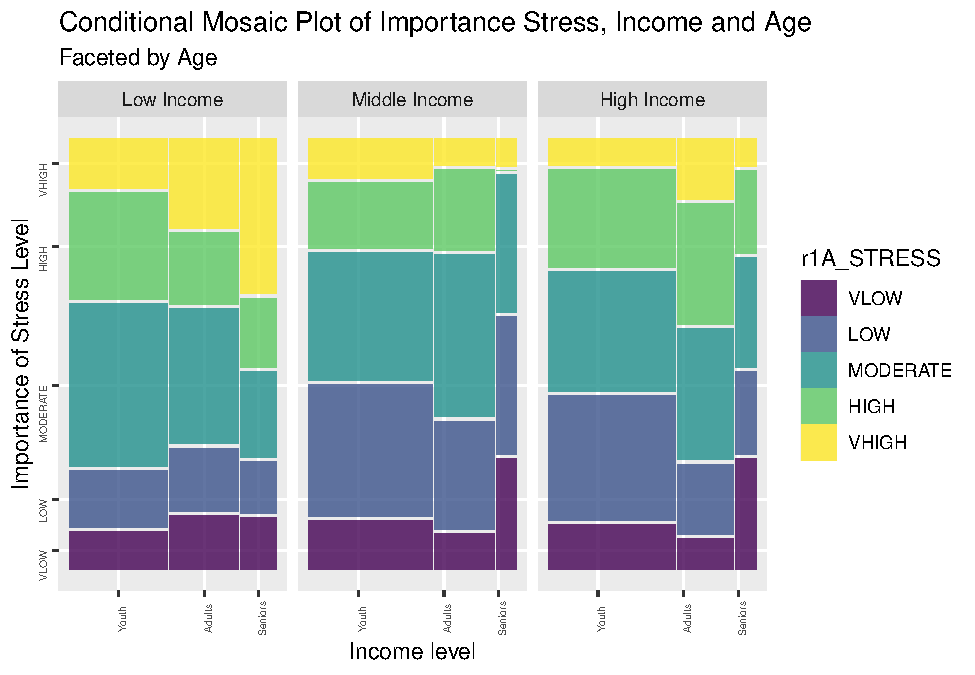
\includegraphics{thesis_files/figure-latex/unnamed-chunk-32-1.pdf}
\caption{\label{fig:unnamed-chunk-32}\label{fig:Income-Age-stress}Conditional Mosaic Plot of Importance Stress, Income and Age}
\end{figure}
The analysis of the data (see Figure \ref{fig:Income-Age-stress}) presents a segmentation of stress levels based on income and age groups. Stress level categorized as ``Very low'' is highly associated with middle-income youth, low-income adults, and high-income seniors. ``Low'' stress level is prevalent among middle-income youth, adults, and seniors. The ``Moderate'' stress category can be seen more among high-income youth and seniors, as well as low-income adults. Stress level categorized as ``High'' is mainly linked to high-income youth, adults, and seniors. Lastly, the ``Very high'' stress category is primarily related to middle-income youth, low-income adults, and seniors. This comprehensive breakdown offers valuable insights into how stress perception is nuanced across distinct income and age groups.

\hypertarget{conclusion}{%
\section{Conclusion}\label{conclusion}}

This study has been conducted to investigate the effect of commuting stress on transport mode of active and motorized travelers along with the coping strategies. Recently, it has been more important in research to evaluate how these consequences are felt by commuters using various modes of transportation, particularly active ones.

Measuring stress entails an individual self-evaluation of a wide variety variables when commuting preferably while commuting. There is a link between stress and commuting in the literature, which takes into account factors such as time commute (Evans \& Wener, 2006), control and predictability (Gottholmseder et al., 2009), as already has been found according to the previous studies about travel motives specially instrumental ones. The component of stress level has a negative connotation in the context of this research (as no one would prefer to be stressed) and investigates the internal mental reaction of the traveler based on their commuting journeys.

In this research we aimed at understanding how stress affect active and motorized travelers' choice of modes by investigating their stress level. Furthermore, we look into the significance that travelers place on their stress levels. This allows us to investigate the concept of ``limited horizons,'' or how those who are less adaptable normalize subpar experiences. The current study on commuting stress is going to address the following questions:

-How crucial it is for respondents to make a journey while feeling a sense of stress and to what scale they are going to evaluate this feeling?

-What elements go into determining how stressed active and motorized travelers are when traveling?

-Can commuters think of normalization and learned helplessness as coping mechanisms? If yes, which category of people.

In order to find out the how people feel stress while commuting, the association between some key exploratory variables and our income variables has been assessed. The study found that while public users assume least importance level, they feel highest level of stress. When we consider a three-way association among active, public and private users, we can see first public and then private users as the more populated groups feel more stress and do not care as much as active users. This result are in the same page with previous work as (Brutus et al., 2017) found those who cycled to work felt less stress than others who commute by motorized modes.

Results also have shown that although public transport is the most popular mode, those who use public transport are mostly low income. These findings echoes results from (Tiznado-Aitken et al., 2021) where they found in Latin America due to some deficiencies of land use planning and transport category of low-income people suffer from long commute between work and home. Because of their status and not having high chance of car ownership, they become captive users of public transport as the fundamental mode of transport.

As been previously indicated, low income people, the least populated group are the most group at the exposure of feeling stress because they are the most interested users of public transport and they do not care about the feeling of stress as much as high and middle income groups. As (Gatersleben \& Uzzell, 2007) also supported previous studies people reported more stressful journeys by car and public transit than active mode due to different sources mainly delays because of traffic jams, behavior of other (car) users, poor infrastructure provision (for public users).

It could be also interesting that the least popular mode is active which also has been mostly used by low income people who are the most careful people about the importance of stress and have undergone the least stress. This echoes the similar findings as (Smith, 2017) has indicated that people who bike and walk to workplace are happier with their commute experience.

One of the reasons behind this fact that active mode has not been used as the most popular in Chile according to (Herrmann-Lunecke, Mora, \& Sagaris, 2020) is the lack of physical safety infrastructure (``walkability'' of the sidewalks). Furthermore, lack of safety in Chile leading to sexual harassment especially for women make them avoid walking and using public transport and stick to taxi even among those with low budget.
As expected in Chile as a developing global south country, while high income cluster are the more interested in using public transport, they can be considered as the most users of private modes of transport. These people are the second most affected group by feeling commuting stress and population after low income people.

Findings have shown that youth who use public transport are mostly youth and they feel highest amount of stress while they assign almost least importance to their feeling compared to other age groups and modes. Also people who are dependent on public transport as the most popular mode, which has already been known as the most stressful mode of transport, care about stress less than any other group and they are mostly youth.

Adults are mostly interested in using private transportation and while they feel less commuting stress than public users, they care about it more than them. Seniors as the least populated group are also similar to adults in terms of getting interested in using private transport and they feel in the same way as adults. It is interesting to note that active transport users include mostly middle and high income youth category who doesn't feel stress that much while commuting but they care about stress more than any other group.

As study has shown, people associated with low income level mostly use public transport feel higher levels of stress while they do not care about that compared to middle income ones who care about their feeling of stress more than any group. These low income people are more youth who are more interested in active and public mode at all income levels but they highest experience of feeling stress is when they are using public and the most peaceful is when they use active mode. Although travel could be stressful but there should be a moderator feeling of normalization for them to overcome this stressful experience (Gustafson, 2014).

Moreover high income people who are more dependent on private mode feel very high level of stress and assign a slight rate of importance to their feeling. This people are also more young and adult commuters.The reason behind why people would stay on their mode of transport choice can be various.

As it has been indicated, respondents in Santiago, Chile are mostly low income and middle income. So they probably do not have enough budget to have access to the mode which is less stressful and efficient. As previous findings (Tironi \& Palacios, 2016) support the fact that some commuters despite of the anxiety and stress experienced by daily travels using ``Transantiago'' (modern public transportation of Santiago), would decide to sell their private car because of financial issues and stay on public transport. When facing the feeling of stress some people can deal with that or to somehow getting used to that experience by repeating more and more to develop a sense of ``travel competence'' arisen from their attempts in reducing travel-related stress and inconvenience on the road.

While normalization can be beneficial in terms of reducing stress, it could lead to make travel less exciting. As in this study we focused mostly on commutes to regular destinations like work, school and so on, we analyzed that these travels come from instrumental motives in which commuters care about their professional goals more than leisure and spare time. For travel to work people consider factors like environment, cost, health and fitness, convenience and predictability flexibility and obviously they feel more stress than in a recreational travel. So, normalization is going to distinguish between normal travel and fun travel. For fun travel people tend to commute to longer and unusual trips which seems more exciting whereas for normal travel all activities may become routine and repetition.

This research demonstrates that the normalization processes possess the capability to moderate and reshape the stressful experiences of travel in various ways. This process can be used as a coping strategy for those who are low income and have poor access to urban facilities, enough budget and lack of urban fairness in Santiago, Chile.

\hypertarget{conclusion-1}{%
\chapter{Conclusion}\label{conclusion-1}}

The knowledge of commuting stress in both psychological context and travel behavior studies is of importance as it tends to have a significant impact on daily patterns of commute. This thesis focuses on analysis of the interaction between urban movements, daily commute, stress feelings towards the travel experiences and their reaction.

Chapter contributes to construct a comprehensive foundation into the format of a data package including a wide variety aspects of living and moving in urban environment. As it has been indicated earlier, people may have different travel experience in terms of perceiving stress and assigning importance to the negative feeling regarding their occupation, age, income and the mode of transportation choice. Second paper includes modelling techniques to understand the interaction between our outcome and exploratory variables to identify how commuters based on different categories are affected and what coping strategies can be applied to them.

In the following sections of this chapter, the mentioned contributions will be discussed in depth along with policy implication of the research, study limitations and further research.

\hypertarget{research-contribution}{%
\section{Research Contribution}\label{research-contribution}}

Research primarily aimed at exploring travel behavior and commuting stress on a daily basis. This thesis also contributes to understanding the copings strategies that may have been used by commuters.

\hypertarget{providing-a-data-package-based-on-travel-behavior-of-santiaguinos-commuters.}{%
\subsection{Providing a data package based on travel behavior of Santiaguinos commuters.}\label{providing-a-data-package-based-on-travel-behavior-of-santiaguinos-commuters.}}

The research has collected a broad range of information based on a large-scale travel survey. This package is a valuable resource as it has been purposefully collected, helpful to understand travel behavior and urban experiences including residential context, demographic information, built environment, work commute behaviors and health and feelings information. The psychological part of the survey helps investigating the mental impacts of travels and health outcomes. This information gives beneficial insights into transportation planning, public sector development and health-related policies.

\hypertarget{influential-attributes-in-commuting-stress-experiences}{%
\subsection{Influential attributes in commuting stress experiences}\label{influential-attributes-in-commuting-stress-experiences}}

Findings based on the bivariate ordinal regression model suggested that people may have different feelings from happiness and excitement to anxiety and stress according to various socio-demographic situations such as different age groups, occupations, income levels and the primary mode of transport choice. In terms of importance of understanding the possible stressors (Useche et al., 2023) found that while commuters encounter daily negative commute experiences such as traffic jams, deficiencies in transport choices, crowded public transport services, prolonged trips, and road conflicts, there are not much studies that have methodologically addressed the issue of commuting stress (CS). Findings of the current study have indicated that mostly pertaining to lower levels of income, young age range, using public modes may cause people to feel more stress while considering not enough importance to that feeling.

\hypertarget{potential-coping-strategies}{%
\subsection{Potential coping strategies}\label{potential-coping-strategies}}

According to the results from the modelling process and exploring the previous studies in terms of the ways that people deal with stress, concept of normalization as an emotion-based coping strategy has been indicated to be employed by commuters. As indicated earlier almost more than half of Santiaguinos are related to middle income and low income and had limited transportation options. As (Chen, 2017) found, work-related travels may be integrated with stress and this negative feeling of travelers can be rationalized and adjusted leading to normalization. In fact, business travelers may experience different level of stress than leisure commuters and they know how to develop their strategies to normalize the stress that they are facing with. Hence, understanding various aspects of work commuters' stressors is important to address their issue associated with commuting stress.

\hypertarget{policy-implications}{%
\section{Policy Implications}\label{policy-implications}}

\hypertarget{invest-in-public-transport-infrastructure}{%
\subsection{Invest in Public Transport Infrastructure}\label{invest-in-public-transport-infrastructure}}

As the results from the modelling process of this dissertation have indicated, almost more than half of the respondents were characterized as middle-income and low-income people who relied on using public mode of transport for daily work commute. The findings also have revealed that although youth age range are the most stress affected commuters out of this people, they did not care about feeling of stress as they were assumed to be. Following this issue, enhancement in public transportation infrastructure could be considered as a crucial policy implication in research. According to commuters' experiences, having access to a more reliable, efficient, and comfortable public transportation can reduce the stress associated with commuting, especially for those who rely on it such as younger people from middle-income and low-income groups in this research. There for policy makers should consider that investments in public transit can lead to reduced congestion, shorter commute times, and a more positive and satisfying commuting experience.

\hypertarget{promote-alternative-transportation-modes}{%
\subsection{Promote Alternative Transportation Modes}\label{promote-alternative-transportation-modes}}

The results of the thesis suggested that active transport modes like walking or cycling is the least popular mode in Santiago. It is interesting that this mode is mostly used by low-income categories who are more conscious of the importance of stress, but experience relatively lower stress levels as opposed to those from the same group but with high stress and interested in public mode. As similar Chilean studies like (Herrmann-Lunecke et al., 2020) have shown the unpopularity of active transportation can be attributed to safety concerns, including sexual harassment, and a lack of safe infrastructure. Thus, encouraging the use of alternative and healthy transport modes like cycling and walking, and even carpooling would be another key policy implication. These modes can reduce the stress of daily commuting, help to promote physical activity, and contribute to environmental sustainability. Hence, policies that create safe and convenient options for active transportation can significantly impact commuters' well-being and reduce commuting stress.

\hypertarget{further-research}{%
\section{Further Research}\label{further-research}}

The research analyzed the impact of stress on commuters on a daily basis by investigating the interaction among experienced stress, importance of that and socio-demographic variables to understand the relevant coping strategies to address this issue. However, there are some other research questions needed further attention.

\hypertarget{exploring-cross-cultural-impacts-on-travel-patterns-and-commuting-stress}{%
\subsection{Exploring Cross-Cultural impacts on travel patterns and commuting stress}\label{exploring-cross-cultural-impacts-on-travel-patterns-and-commuting-stress}}

Understanding the cross-cultural differences in commuting stress and coping strategies can be helpful in studying how individuals in different cultural contexts experience and manage their stress associated with their daily commutes. Furthermore, it can be explored whether various cultural factors, such as societal norms and lifestyles, values, and communication styles, influence how people perceive and cope with commuting stress. For instance, (Balbontin et al., 2021) has investigated the cross-cultural comparisons using data in eight countries (Argentina, Australia, Brazil, Chile, Colombia, Ecuador, Peru and South Africa). They explored the incidence of remote working post-COVID-19 and what impact this could have on the number of weekly commuting trips. Therefore, exploring the changes in travel behavior and commuting stress due to various reasons and in different cultural context would be beneficial in understanding and prediction of new trends.

\hypertarget{the-role-of-technology-in-commuting}{%
\subsection{The Role of Technology in Commuting}\label{the-role-of-technology-in-commuting}}

According to the literature review in this research, people differ from employing a technique to deal with their stressful experience of commuting. Some of them may take an advantage of problem-focused and other ones would be interested in using emotion-focused coping strategies. As a result, further research area could investigate the role of technology in modern commuting experiences, including the impact of digital gadgets and interventions in the way that people deal with the negative feeling when traveling. Regarding the increasing use of technology in daily life, understanding commuters' interactions with these digital tools during the travel is of importance. As (Holden \& Sunindijo, 2018) has pointed out while stress can have negative effect on work-life balance, technology would have an improving role on that. For example, people can undertake their job responsibilities using a phone, avoid commuting stress, allocating their time to other activities and managing both work and life commitments in a more flexible way.

\hypertarget{impacts-of-environmental-factors-on-commuting-experiences}{%
\subsection{Impacts of Environmental Factors on Commuting Experiences}\label{impacts-of-environmental-factors-on-commuting-experiences}}

According to the Santiago data set as a foundation for further analysis, sections of built environment and nature and sustainability of the city people reveal different viewpoints about the effect of physical environment of commuting routes and individuals' experiences during their commutes. Investigating an appropriate way to manage the problem of stress requires further research and development of appropriate interventions. As (Rowden, Matthews, Watson, \& Biggs, 2011) have suggested, interventions may aim at environmental factors such as traffic congestion, mitigating stress responses (e.g., work-related stress management programs), or enhancing the driver's ability to cope with challenges during the commute.

\hypertarget{study-limitations}{%
\section{Study Limitations}\label{study-limitations}}

There are some main limitations in this study should be considered. First there was a shortage in stress specific and objective stressors variables in our data set such as speed, level of traffic congestion, commute starting and ending times, commute duration and so on. Having comprehensive collected data can provide a better understanding of how commuting stress affects commuters and what type of coping strategies they tend to employ.

Second is lack of variation in coping strategy identification in terms of introducing specific coping strategies regarding each mode of transportation. As the research focused on the most affect group of people who were public transport commuters, other significant modes like private ones were excluded while public commuters had negative feelings of stress during their commute.

Third one is related to the collection date of data set used as a foundation for the second paper. The survey conducted a couple of years ago when there was no impact of COVID-19 on travel behavior of Santiaguinos. COVID-19 has significant impacts in terms of changing travel patterns as a notable portion of people have transitioned to remote job or some other have reduced their dependency on using public transportation. Therefore, incorporating COVID-19 related variables will be helpful in providing a more accurate insight into travel behavior and health and safety concerns.

\hypertarget{closing-remarks}{%
\section{Closing remarks}\label{closing-remarks}}

This thesis aimed at investigating the effect of stress on commuting experience of motorized and non motorized commuters and how they address their negative feelings. As study has indicated understanding mode of transport choice and income level would be important as these variables have impact on the stress level during the commute. Public transport users, who are mostly low-income individuals, experience the highest levels of commuting stress. This category of commuters seems to be more resilient to stress, perhaps because of the necessity of using public transport regarding their financial status despite its drawbacks. In contrast, private transport users who are mainly high-income, also face substantial stress, indicating that higher income does not necessarily mean to experience a stress-free commuting. (Evans, Wener, \& Phillips, 2002) also pointed an interesting explanation about role of the degree of predictability as a salient contributor to commuting stress in commuter mode selection. Perhaps private mode users are more interested in using their own vehicle than public means of transportation because they feel more predictability than mass transit options.

Thesis also has investigated the role of normalization as a coping mechanism. The concept of ``limited horizons'' and normalization appear as a well-fitted coping mechanism. Low-income commuters, despite undergoing high stress levels, reveal a level of adaptation or normalization, possibly resulting from their reliance on public transport. This normalization process has been indicated to be beneficial for them to deal with daily stressors associated with commuting.

Age as another influential demographic characteristics on stress perception has been reviewed in this study. Younger commuters, especially those relying on public transport, have reported the highest stress levels but have assigned the least importance to their negative feelings. This generation seems to be more resilient or indifferent to commuting stress comparing to their counterparts. Contrastingly, adults as a category who are primarily using private transport, have undergone less stress but they have prioritized addressing it, revealing a greater concern for their well-being.

These findings emphasize the complex interaction among socioeconomic factors, mode of transport choice, and stress perception in the context of daily commuting. Furthermore, the importance of considering psychological aspects and adhering to them as coping strategies, such as normalization has been indicated when it comes to designing policies and interventions to enhance commuting experiences and feelings. Understanding these dynamics can inform policymakers and transportation planners as they work towards creating a more equitable, efficient, and less stressful transportation systems. For instance, (Smith, 2017) has indicated that policymakers should continue make active travel options more available as people feel more happier commuting by bike or walk. Future research could delve deeper into the decent coping mechanisms employed by different commuter groups and explore how these findings can be used in other global contexts.

\backmatter

\hypertarget{references}{%
\chapter*{References}\label{references}}
\addcontentsline{toc}{chapter}{References}

\markboth{References}{References}

\noindent

\setlength{\parindent}{-0.20in}
\setlength{\leftskip}{0.20in}
\setlength{\parskip}{8pt}

\hypertarget{refs}{}
\begin{CSLReferences}{1}{0}
\leavevmode\vadjust pre{\hypertarget{ref-abou2012happiness}{}}%
Abou-Zeid, M., Witter, R., Bierlaire, M., Kaufmann, V., \& Ben-Akiva, M. (2012). Happiness and travel mode switching: Findings from a swiss public transportation experiment. \emph{Transport Policy}, \emph{19}(1), 93--104.

\leavevmode\vadjust pre{\hypertarget{ref-alyavina2020mobility}{}}%
Alyavina, E., Nikitas, A., \& Njoya, E. T. (2020). Mobility as a service and sustainable travel behaviour: A thematic analysis study. \emph{Transportation Research Part F: Traffic Psychology and Behaviour}, \emph{73}, 362--381.

\leavevmode\vadjust pre{\hypertarget{ref-anable2005all}{}}%
Anable, J., \& Gatersleben, B. (2005). All work and no play? The role of instrumental and affective factors in work and leisure journeys by different travel modes. \emph{Transportation Research Part A: Policy and Practice}, \emph{39}(2-3), 163--181.

\leavevmode\vadjust pre{\hypertarget{ref-babore2020psychological}{}}%
Babore, A., Lombardi, L., Viceconti, M. L., Pignataro, S., Marino, V., Crudele, M., \ldots{} Trumello, C. (2020). Psychological effects of the COVID-2019 pandemic: Perceived stress and coping strategies among healthcare professionals. \emph{Psychiatry Research}, \emph{293}, 113366.

\leavevmode\vadjust pre{\hypertarget{ref-balbontin2021impact}{}}%
Balbontin, C., Hensher, D. A., Beck, M. J., Giesen, R., Basnak, P., Vallejo-Borda, J. A., \& Venter, C. (2021). Impact of COVID-19 on the number of days working from home and commuting travel: A cross-cultural comparison between australia, south america and south africa. \emph{Journal of Transport Geography}, \emph{96}, 103188.

\leavevmode\vadjust pre{\hypertarget{ref-benyamini2017normalization}{}}%
Benyamini, Y., Gozlan, M., \& Weissman, A. (2017). Normalization as a strategy for maintaining quality of life while coping with infertility in a pronatalist culture. \emph{International Journal of Behavioral Medicine}, \emph{24}, 871--879.

\leavevmode\vadjust pre{\hypertarget{ref-boran2022psychological}{}}%
Boran, M., Boran, O. F., Korukcu, O., \& Özkaya, M. (2022). The psychological resilience and perceived stress of the frontline heroes in the pandemic in turkey: A descriptive study of the COVID-19 outbreak-mutations-normalization triad. \emph{Japan Journal of Nursing Science}, \emph{19}(1), e12442.

\leavevmode\vadjust pre{\hypertarget{ref-brutus2017cycling}{}}%
Brutus, S., Javadian, R., \& Panaccio, A. J. (2017). Cycling, car, or public transit: A study of stress and mood upon arrival at work. \emph{International Journal of Workplace Health Management}, \emph{10}(1), 13--24.

\leavevmode\vadjust pre{\hypertarget{ref-chatterjee2020commuting}{}}%
Chatterjee, K., Chng, S., Clark, B., Davis, A., De Vos, J., Ettema, D., \ldots{} Reardon, L. (2020). Commuting and wellbeing: A critical overview of the literature with implications for policy and future research. \emph{Transport Reviews}, \emph{40}(1), 5--34.

\leavevmode\vadjust pre{\hypertarget{ref-chen2017travel}{}}%
Chen, H. S. (2017). Travel well, road warriors: Assessing business travelers' stressors. \emph{Tourism Management Perspectives}, \emph{22}, 1--6.

\leavevmode\vadjust pre{\hypertarget{ref-ellder2020telework}{}}%
Elldér, E. (2020). Telework and daily travel: New evidence from sweden. \emph{Journal of Transport Geography}, \emph{86}, 102777.

\leavevmode\vadjust pre{\hypertarget{ref-ettema2011satisfaction}{}}%
Ettema, D., Gärling, T., Eriksson, L., Friman, M., Olsson, L. E., \& Fujii, S. (2011). Satisfaction with travel and subjective well-being: Development and test of a measurement tool. \emph{Transportation Research Part F: Traffic Psychology and Behaviour}, \emph{14}(3), 167--175.

\leavevmode\vadjust pre{\hypertarget{ref-evans2006rail}{}}%
Evans, G. W., \& Wener, R. E. (2006). Rail commuting duration and passenger stress. \emph{Health Psychology}, \emph{25}(3), 408.

\leavevmode\vadjust pre{\hypertarget{ref-evans2002morning}{}}%
Evans, G. W., Wener, R. E., \& Phillips, D. (2002). The morning rush hour: Predictability and commuter stress. \emph{Environment and Behavior}, \emph{34}(4), 521--530.

\leavevmode\vadjust pre{\hypertarget{ref-folkman1985if}{}}%
Folkman, S., \& Lazarus, R. S. (1985). If it changes it must be a process: Study of emotion and coping during three stages of a college examination. \emph{Journal of Personality and Social Psychology}, \emph{48}(1), 150.

\leavevmode\vadjust pre{\hypertarget{ref-gardner2007drives}{}}%
Gardner, B., \& Abraham, C. (2007). What drives car use? A grounded theory analysis of commuters' reasons for driving. \emph{Transportation Research Part F: Traffic Psychology and Behaviour}, \emph{10}(3), 187--200.

\leavevmode\vadjust pre{\hypertarget{ref-gatersleben2007affective}{}}%
Gatersleben, B., \& Uzzell, D. (2007). Affective appraisals of the daily commute: Comparing perceptions of drivers, cyclists, walkers, and users of public transport. \emph{Environment and Behavior}, \emph{39}(3), 416--431.

\leavevmode\vadjust pre{\hypertarget{ref-gomez2023urban}{}}%
Gómez-Lobo, A., \& Micco, A. (2023). Urban commuting time and sick-leave medical license use: An empirical study of santiago, chile. \emph{Economics of Transportation}, \emph{33}, 100287.

\leavevmode\vadjust pre{\hypertarget{ref-gottholmseder2009stress}{}}%
Gottholmseder, G., Nowotny, K., Pruckner, G. J., \& Theurl, E. (2009). Stress perception and commuting. \emph{Health Economics}, \emph{18}(5), 559--576.

\leavevmode\vadjust pre{\hypertarget{ref-gustafson2014business}{}}%
Gustafson, P. (2014). Business travel from the traveller's perspective: Stress, stimulation and normalization. \emph{Mobilities}, \emph{9}(1), 63--83.

\leavevmode\vadjust pre{\hypertarget{ref-herrmann2020persistence}{}}%
Herrmann-Lunecke, M. G., Mora, R., \& Sagaris, L. (2020). Persistence of walking in chile: Lessons for urban sustainability. \emph{Transport Reviews}, \emph{40}(2), 135--159.

\leavevmode\vadjust pre{\hypertarget{ref-herrmann2021perception}{}}%
Herrmann-Lunecke, M. G., Mora, R., \& Vejares, P. (2021). Perception of the built environment and walking in pericentral neighbourhoods in santiago, chile. \emph{Travel Behaviour and Society}, \emph{23}, 192--206.

\leavevmode\vadjust pre{\hypertarget{ref-hill2007driver}{}}%
Hill, J. D., \& Boyle, L. N. (2007). Driver stress as influenced by driving maneuvers and roadway conditions. \emph{Transportation Research Part F: Traffic Psychology and Behaviour}, \emph{10}(3), 177--186.

\leavevmode\vadjust pre{\hypertarget{ref-hirk2020mvord}{}}%
Hirk, R., Hornik, K., \& Gür, L. V. (2020). Mvord: An r package for fitting multivariate ordinal regression models. \emph{Journal of Statistical Software}, \emph{93}(4), 1--41.

\leavevmode\vadjust pre{\hypertarget{ref-holden2018technology}{}}%
Holden, S., \& Sunindijo, R. Y. (2018). Technology, long work hours, and stress worsen work-life balance in the construction industry. \emph{International Journal of Integrated Engineering}, \emph{10}(2).

\leavevmode\vadjust pre{\hypertarget{ref-iwasaki2005gender}{}}%
Iwasaki, Y., MacKay, K., \& Mactavish, J. (2005). Gender-based analyses of coping with stress among professional managers: Leisure coping and non-leisure coping. \emph{Journal of Leisure Research}, \emph{37}(1), 1--28.

\leavevmode\vadjust pre{\hypertarget{ref-jamal2020perceptions}{}}%
Jamal, S., Mohiuddin, H., \& Paez, A. (2020). How do the perceptions of neighborhood conditions impact active transportation? A study in rajshahi, bangladesh. \emph{Transportation Research Part D: Transport and Environment}, \emph{87}, 102525.

\leavevmode\vadjust pre{\hypertarget{ref-kenne2016pairwise}{}}%
Kenne Pagui, E. C., \& Canale, A. (2016). Pairwise likelihood inference for multivariate ordinal responses with applications to customer satisfaction. \emph{Applied Stochastic Models in Business and Industry}, \emph{32}(2), 273--282.

\leavevmode\vadjust pre{\hypertarget{ref-kontogiannis2006patterns}{}}%
Kontogiannis, T. (2006). Patterns of driver stress and coping strategies in a greek sample and their relationship to aberrant behaviors and traffic accidents. \emph{Accident Analysis \& Prevention}, \emph{38}(5), 913--924.

\leavevmode\vadjust pre{\hypertarget{ref-koslowsky1997commuting}{}}%
Koslowsky, M. (1997). Commuting stress: Problems of definition and variable identification. \emph{Applied Psychology: An International Review}.

\leavevmode\vadjust pre{\hypertarget{ref-koslowsky2013commuting}{}}%
Koslowsky, M., Kluger, A. N., \& Reich, M. (2013). \emph{Commuting stress: Causes, effects, and methods of coping}. Springer Science \& Business Media.

\leavevmode\vadjust pre{\hypertarget{ref-legrain2015stressed}{}}%
Legrain, A., Eluru, N., \& El-Geneidy, A. M. (2015). Am stressed, must travel: The relationship between mode choice and commuting stress. \emph{Transportation Research Part F: Traffic Psychology and Behaviour}, \emph{34}, 141--151.

\leavevmode\vadjust pre{\hypertarget{ref-loosemore2004gender}{}}%
Loosemore, M., \& Waters, T. (2004). Gender differences in occupational stress among professionals in the construction industry. \emph{Journal of Management in Engineering}, \emph{20}(3), 126--132.

\leavevmode\vadjust pre{\hypertarget{ref-lowe2016conceptual}{}}%
Lowe, K., \& Mosby, K. (2016). The conceptual mismatch: A qualitative analysis of transportation costs and stressors for low-income adults. \emph{Transport Policy}, \emph{49}, 1--8.

\leavevmode\vadjust pre{\hypertarget{ref-maier1976learned}{}}%
Maier, S. F., \& Seligman, M. E. (1976). Learned helplessness: Theory and evidence. \emph{Journal of Experimental Psychology: General}, \emph{105}(1), 3.

\leavevmode\vadjust pre{\hypertarget{ref-mattisson2018modelling}{}}%
Mattisson, K., Idris, A. O., Cromley, E., Håkansson, C., Östergren, P.-O., \& Jakobsson, K. (2018). Modelling the association between health indicators and commute mode choice: A cross-sectional study in southern sweden. \emph{Journal of Transport \& Health}, \emph{11}, 110--121.

\leavevmode\vadjust pre{\hypertarget{ref-mokhtarian2001derived}{}}%
Mokhtarian, P. L., \& Salomon, I. (2001). How derived is the demand for travel? Some conceptual and measurement considerations. \emph{Transportation Research Part A: Policy and Practice}, \emph{35}(8), 695--719.

\leavevmode\vadjust pre{\hypertarget{ref-munoz2008transantiago}{}}%
Muñoz, J. C., \& Gschwender, A. (2008). Transantiago: A tale of two cities. \emph{Research in Transportation Economics}, \emph{22}(1), 45--53.

\leavevmode\vadjust pre{\hypertarget{ref-nakano1991role}{}}%
Nakano, K. (1991). The role of coping strategies on psychological and physical well-being. \emph{Japanese Psychological Research}, \emph{33}(4), 160--167.

\leavevmode\vadjust pre{\hypertarget{ref-novaco2009commuting}{}}%
Novaco, R. W., \& Gonzalez, O. I. (2009). Commuting and well-being. \emph{Technology and Well-Being}, \emph{3}, 174--4.

\leavevmode\vadjust pre{\hypertarget{ref-odufuwa2008gender}{}}%
Odufuwa, B. (2008). Gender differentials, vulnerability and mobility stress coping strategies in nigeria. \emph{Journal of Geography and Regional Planning}, \emph{1}(7), 132.

\leavevmode\vadjust pre{\hypertarget{ref-paez2010enjoyment}{}}%
Páez, A., \& Whalen, K. (2010). Enjoyment of commute: A comparison of different transportation modes. \emph{Transportation Research Part A: Policy and Practice}, \emph{44}(7), 537--549.

\leavevmode\vadjust pre{\hypertarget{ref-pezoa2023estimation}{}}%
Pezoa, R., Basso, F., Quilodrán, P., \& Varas, M. (2023). Estimation of trip purposes in public transport during the COVID-19 pandemic: The case of santiago, chile. \emph{Journal of Transport Geography}, \emph{109}, 103594.

\leavevmode\vadjust pre{\hypertarget{ref-rabbitt1990age}{}}%
Rabbitt, P. (1990). Age, IQ and awareness, and recall of errors. \emph{Ergonomics}, \emph{33}(10-11), 1291--1305.

\leavevmode\vadjust pre{\hypertarget{ref-rana2020mental}{}}%
Rana, W., Mukhtar, S., \& Mukhtar, S. (2020). Mental health of medical workers in pakistan during the pandemic COVID-19 outbreak. \emph{Asian Journal of Psychiatry}, \emph{51}, 102080.

\leavevmode\vadjust pre{\hypertarget{ref-rowden2011relative}{}}%
Rowden, P., Matthews, G., Watson, B., \& Biggs, H. (2011). The relative impact of work-related stress, life stress and driving environment stress on driving outcomes. \emph{Accident Analysis \& Prevention}, \emph{43}(4), 1332--1340.

\leavevmode\vadjust pre{\hypertarget{ref-sha2019beyond}{}}%
Sha, F., Li, B., Law, Y. W., \& Yip, P. S. (2019). Beyond the resource drain theory: Salary satisfaction as a mediator between commuting time and subjective well-being. \emph{Journal of Transport \& Health}, \emph{15}, 100631.

\leavevmode\vadjust pre{\hypertarget{ref-shamoa2010aggression}{}}%
Shamoa-Nir, L., \& Koslowsky, M. (2010). Aggression on the road as a function of stress, coping strategies and driver style. \emph{Psychology}, \emph{1}, 35--44.

\leavevmode\vadjust pre{\hypertarget{ref-smith2017commute}{}}%
Smith, O. (2017). Commute well-being differences by mode: Evidence from portland, oregon, USA. \emph{Journal of Transport \& Health}, \emph{4}, 246--254.

\leavevmode\vadjust pre{\hypertarget{ref-tironi2016affects}{}}%
Tironi, M., \& Palacios, R. (2016). Affects and urban infrastructures: Researching users' daily experiences of santiago de chile's transport system. \emph{Emotion, Space and Society}, \emph{21}, 41--49.

\leavevmode\vadjust pre{\hypertarget{ref-tiznado2021public}{}}%
Tiznado-Aitken, I., Muñoz, J. C., \& Hurtubia, R. (2021). Public transport accessibility accounting for level of service and competition for urban opportunities: An equity analysis for education in santiago de chile. \emph{Journal of Transport Geography}, \emph{90}, 102919.

\leavevmode\vadjust pre{\hypertarget{ref-useche2023another}{}}%
Useche, S. A., Marin, C., \& Llamazares, F. J. (2023). {``Another (hard) day moving in the city''}: Development and validation of the MCSS, a multimodal commuting stress scale. \emph{Transportation Research Part F: Traffic Psychology and Behaviour}, \emph{95}, 143--159.

\leavevmode\vadjust pre{\hypertarget{ref-webster2016fight}{}}%
Webster, V., Brough, P., \& Daly, K. (2016). Fight, flight or freeze: Common responses for follower coping with toxic leadership. \emph{Stress and Health}, \emph{32}(4), 346--354.

\leavevmode\vadjust pre{\hypertarget{ref-wener2011comparing}{}}%
Wener, R. E., \& Evans, G. W. (2011). Comparing stress of car and train commuters. \emph{Transportation Research Part F: Traffic Psychology and Behaviour}, \emph{14}(2), 111--116.

\leavevmode\vadjust pre{\hypertarget{ref-westerman2000individual}{}}%
Westerman, S., \& Haigney, D. (2000). Individual differences in driver stress, error and violation. \emph{Personality and Individual Differences}, \emph{29}(5), 981--998.

\leavevmode\vadjust pre{\hypertarget{ref-ye2019determinants}{}}%
Ye, R., \& Titheridge, H. (2019). The determinants of commuting satisfaction in low-income population: A case study of xi???an, china. \emph{Travel Behaviour and Society}, \emph{16}, 272--283.

\end{CSLReferences}
\end{document}
